%%%% Proceedings format for most of ACM conferences (with the exceptions listed below) and all ICPS volumes.
\documentclass[sigconf]{acmart}
%%%% As of March 2017, [siggraph] is no longer used. Please use sigconf (above) for SIGGRAPH conferences.

%%%% Proceedings format for SIGPLAN conferences 
% \documentclass[sigplan, anonymous, review]{acmart}

%%%% Proceedings format for SIGCHI conferences
% \documentclass[sigchi, review]{acmart}

%%%% To use the SIGCHI extended abstract template, please visit
% https://www.overleaf.com/read/zzzfqvkmrfzn

%%
%% \BibTeX command to typeset BibTeX logo in the docs
\AtBeginDocument{%
  \providecommand\BibTeX{{%
    \normalfont B\kern-0.5em{\scshape i\kern-0.25em b}\kern-0.8em\TeX}}}

%%
%% Submission ID.
%% Use this when submitting an article to a sponsored event. You'll
%% receive a unique submission ID from the organizers
%% of the event, and this ID should be used as the parameter to this command.
\acmSubmissionID{rt1486p}

%%
%% The majority of ACM publications use numbered citations and
%% references.  The command \citestyle{authoryear} switches to the
%% "author year" style.
%%
%% If you are preparing content for an event
%% sponsored by ACM SIGGRAPH, you must use the "author year" style of
%% citations and references.
%% Uncommenting
%% the next command will enable that style.
%%\citestyle{acmauthoryear}


%% My Preamble
\usepackage{graphicx}
\renewcommand{\citename}{\citet}
\renewcommand{\cite}{\citep}


% For maths
\usepackage{amssymb}

% For algorithms
\usepackage{StyFiles/algorithm}
\usepackage{StyFiles/algorithmic}

% My macros
\usepackage{StyFiles/sg-macros}

\newcommand{\mmqp}[3]{\textrm{\sc MaxMarginQP}\!\left(\{\by_t, #1\}_{t=1}^{T}, #2, #3\right)}

% MISC
\usepackage{textcomp}
\usepackage{makecell}
\usepackage{booktabs}
\usepackage{multirow}

%%
%% end of the preamble, start of the body of the document source.
\begin{document}

%% Rights management information.  This information is sent to you
%% when you complete the rights form.  These commands have SAMPLE
%% values in them; it is your responsibility as an author to replace
%% the commands and values with those provided to you when you
%% complete the rights form.
\copyrightyear{2019} 
\acmYear{2019} 
\setcopyright{acmcopyright}
\acmConference[KDD '19]{The 25th ACM SIGKDD Conference on Knowledge Discovery and Data Mining}{August 4--8, 2019}{Anchorage, AK, USA}
\acmBooktitle{The 25th ACM SIGKDD Conference on Knowledge Discovery and Data Mining (KDD '19), August 4--8, 2019, Anchorage, AK, USA}
\acmPrice{15.00}
\acmDOI{10.1145/3292500.3330983}
\acmISBN{978-1-4503-6201-6/19/08}

\settopmatter{printacmref=true}
\fancyhead{}

%%
%% The "title" command has an optional parameter,
%% allowing the author to define a "short title" to be used in page headers.
\title[Multi-task RNN and Higer-order MRFs for Stock Price
Classification]{Multi-task Recurrent Neural Networks and Higher-order
  Markov Random Fields for Stock Price Movement
  Prediction}

%%
%% The "author" command and its associated commands are used to define
%% the authors and their affiliations.
%% Of note is the shared affiliation of the first two authors, and the
%% "authornote" and "authornotemark" commands
%% used to denote shared contribution to the research.
\author{Chang Li}
\affiliation{%
  \institution{UBTECH Sydney AI Centre, SCS, University of Sydney}
  \institution{Capital Markets CRC, Australia}
}
\email{chli4934@uni.sydney.edu.au}

\author{Dongjin Song${}^{*}$}\thanks {*Dongjin Song and Dacheng Tao are corresponding authors.}

\affiliation{%
  \institution{NEC Laboratories America, Inc.}
}
\email{dsong@nec-labs.com}

\author{Dacheng Tao${}^{*}$}
\affiliation{%
  \institution{UBTECH Sydney AI Centre, SCS, University of Sydney}
}
\email{dacheng.tao@sydney.edu.au}




%%
%% By default, the full list of authors will be used in the page
%% headers. Often, this list is too long, and will overlap
%% other information printed in the page headers. This command allows
%% the author to define a more concise list
%% of authors' names for this purpose.
\renewcommand{\shortauthors}{Li, et al.}

%%
%% The abstract is a short summary of the work to be presented in the
%% article.
\begin{abstract}
  Stock price movement not only depends on the history of individual stock
  movements, but also complex hidden dynamics
  associated with other correlated stocks. Despite the substantial
  effort made to understand the principles of
  stock price movement, few attempts have been made to predict movement
  direction based upon a single stock's historical records together
  with its correlated stocks. Here, we present a multi-task
  recurrent neural network (RNN) with high-order Markov random
  fields (MRFs) to predict stock price movement direction. 
  Specifically, we first design a multi-task RNN
  framework to extract informative features from the raw market
  data of individual stocks without considering any domain
  knowledge. Next, we employ binary MRFs with unary features and
  weighted lower linear envelopes as the higher-order energy
  function to capture higher-order consistency within the
  same stock clique (group). We also derive a latent
  structural SVM algorithm to learn higher-order MRFs in a
  polynomial number of iterations. Finally, a sub-gradient
  algorithm is employed to perform end-to-end training of the RNN and
  high-order MRFs. We conduct thorough empirical studies
  on three popular Chinese stock market indexes and the proposed
  method outperforms baseline approaches. To our best
  knowledge, the proposed technique is the first to
  investigate intra-clique relationships with higher-order MRFs
  for stock price movement prediction.
\end{abstract}

%% todo
%% The code below is generated by the tool at http://dl.acm.org/ccs.cfm.
%% Please copy and paste the code instead of the example below.
%%

%\begin{CCSXML}
%<ccs2012>
%<concept>
%<concept_id>10010147.10010257.10010258.10010262</concept_id>
%<concept_desc>Computing methodologies~Multi-task learning</concept_desc>
%<concept_significance>500</concept_significance>
%</concept>
%<concept>
%<concept_id>10010147.10010257.10010293</concept_id>
%<concept_desc>Computing methodologies~Machine learning approaches</concept_desc>
%<concept_significance>500</concept_significance>
%</concept>
%<concept>
%<concept_id>10010147.10010257.10010293.10010294</concept_id>
%<concept_desc>Computing methodologies~Neural networks</concept_desc>
%<concept_significance>500</concept_significance>
%</concept>
%<concept>
%<concept_id>10010147.10010257.10010293.10010300</concept_id>
%<concept_desc>Computing methodologies~Learning in probabilistic graphical models</concept_desc>
%<concept_significance>500</concept_significance>
%</concept>
%<concept>
%<concept_id>10010147.10010257.10010293.10010300.%10010305</concept_id>
%<concept_desc>Computing methodologies~Latent %variable models</concept_desc>
%<concept_significance>500</concept_significance>
%</concept>
%<concept>
%<concept_id>10010147.10010257.10010293.10010319<%/concept_id>
%<concept_desc>Computing methodologies~Learning %latent representations</concept_desc>
%<concept_significance>500</concept_significance>
%</concept>
%</ccs2012>
%\end{CCSXML}

%\ccsdesc[500]{Computing methodologies~Multi-task learning}
%\ccsdesc[500]{Computing methodologies~Machine learning approaches}
%\ccsdesc[500]{Computing methodologies~Neural networks}
%\ccsdesc[500]{Computing methodologies~Learning in probabilistic graphical models}
%\ccsdesc[500]{Computing methodologies~Latent variable models}
%\ccsdesc[500]{Computing methodologies~Learning latent representations}

%%
%% Keywords. The author(s) should pick words that accurately describe
%% the work being presented. Separate the keywords with commas.



\keywords{ Deep learning, Graphical model, Multivariate time
  series prediction}

% %% A "teaser" image appears between the author and affiliation
% %% information and the body of the document, and typically spans the
% %% page.
% \begin{teaserfigure}
%   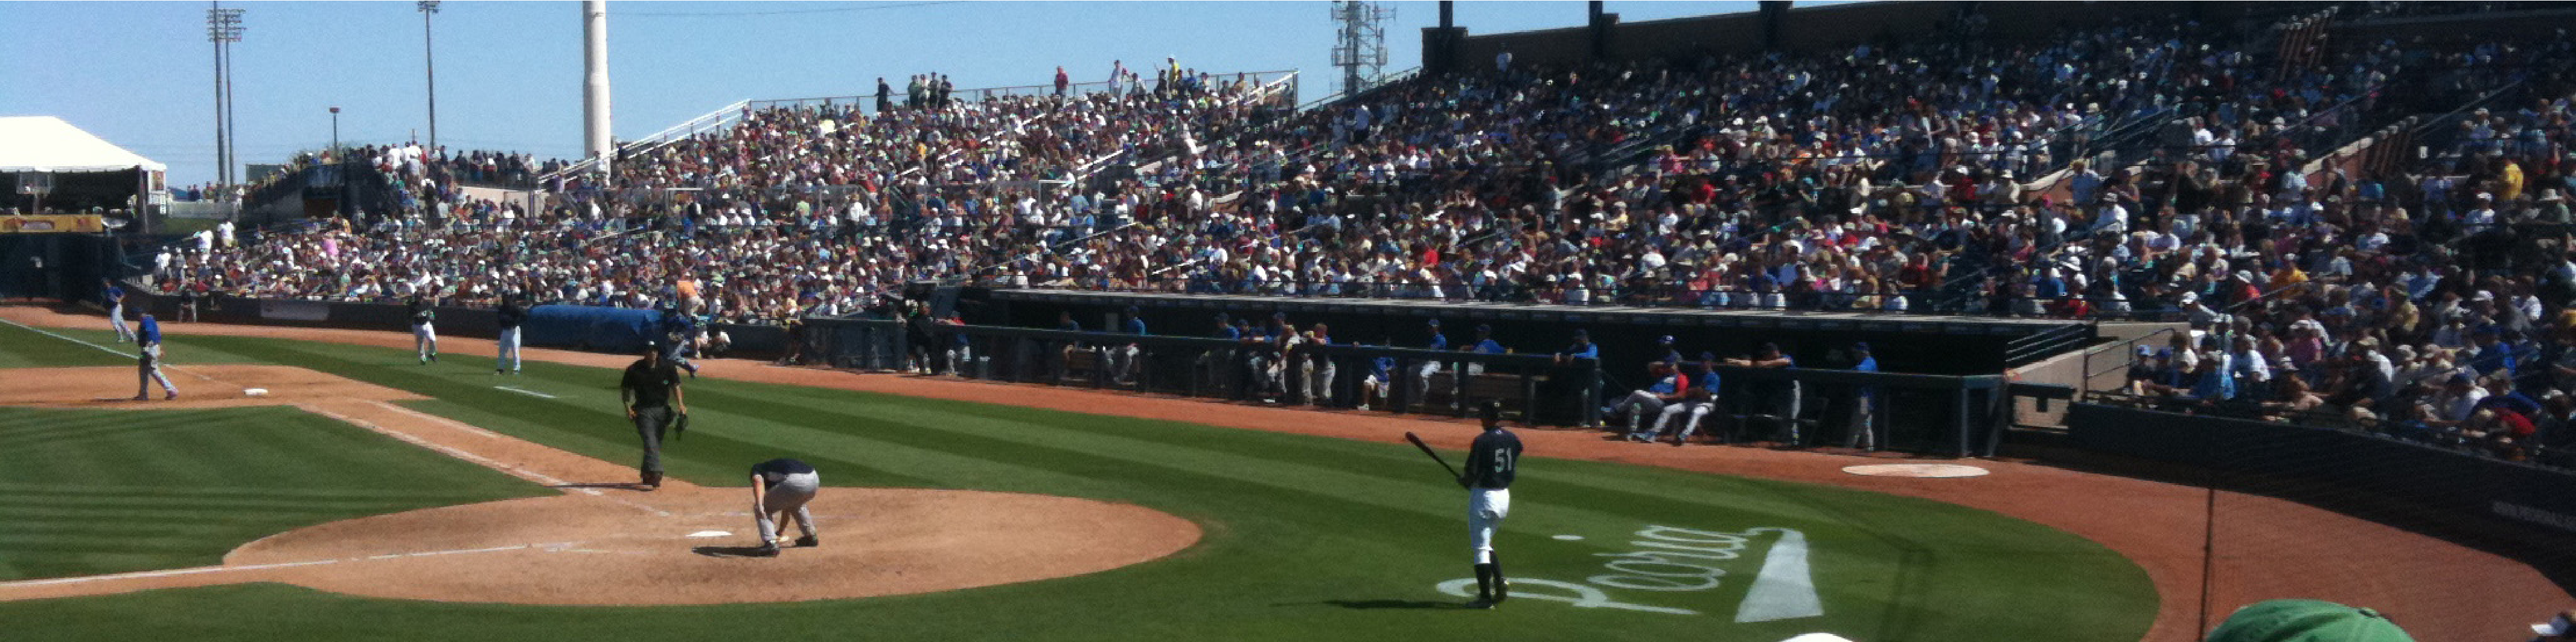
\includegraphics[width=\textwidth]{sampleteaser}
%   \caption{Seattle Mariners at Spring Training, 2010.}
%   \Description{Enjoying the baseball game from the third-base
%   seats. Ichiro Suzuki preparing to bat.}
%   \label{fig:teaser}
% \end{teaserfigure}

%%
%% This command processes the author and affiliation and title
%% information and builds the first part of the formatted document.
\maketitle




\section{Introduction}
\label{sec:intro}
% lead lag 现象不是一直存在,个股趋势也非常重要

It is well known that single the price movement of an individual stock not
only depends on historical records but also highly
correlated to other
stocks~\cite{lo1990contrarian,mech1993portfolio} and may change
in a non-synchronous
manner~\cite{lo1990contrarian,brennan1993investment}. This
correlated yet asynchronous price movement is
sometimes referred to as the lead-lag relationship~\cite{hou2007industry}
between a group of stocks and is thought to arise from the different speed of information
diffusion\cite{lo1990contrarian,badrinath1995shepherds,mcqueen1996delayed}.
When new information hits the market, some stocks
react faster than others and identification
of these leading stocks and their lead-lag relationships to other
lagging stocks provides strong predictive evidence to the
latter\textquotesingle s price movement.

However, there are three key challenges in utilizing the lead-lag
relationship: (1) discovering which stock will be affected by
newly arriving information (such as news); (2) identifying the
group ($e.g.$, industry, supply chain, $etc.$) it belongs to along with
the leading and lagging stocks in this group and
modeling their relationships; (3) predicting the price movement of
each stock by jointly considering knowledge in the correlated
group and an individual stock\textquotesingle price movement at
that moment.

The first challenge is extremely difficult, not only because it
requires an expert level of understanding of the finance system and
market dynamics and the stock price, but also
due to a lack of training data. However, according to the
efficient market
hypothesis~\cite{malkiel1970efficient}, stock price reflects all
available market information.
% chli_comment
% Therefore, informative stock price
% changes can be employed as an approximate of market news arrival.
% In this way, the complexity of the first challenge is transformed
% to the detection of informative price changes in individual
% stocks.
%
Economists hitherto to used patterns hidden inside historical
trading prices and volume to predict future price
movements~\cite{fama1966filter,jensen1967random}. As a result,
hundreds of hand-crafted features, known as technical analysis
indicators~\cite{kirkpatrick2010technical}, have been designed.
However, most of these models have stopped generating profitable
signals since the early 1990s~\cite{park2007we}.
% chli_comment Since trading strategies based on technical
% analysis rules are publicly available and easy to replicate,
% informed institutional traders have been motivated to
% manipulate the market price and encourage retail (individual)
% traders to follow their manipulated price to generate excess
% profit~\cite{sun2016decision}.

To overcome these problems and address the first challenge, here
we employ an end-to-end hierarchical
multi-task~\cite{caruana1993multitask} RNN to extract informative
changes from raw market prices without using hand-crafted
features such as technical analysis indicators. Good price
prediction relies on rich representations and a multi-task
framework that can leverage complementary aspects from diverse
tasks~\cite{sogaard2016deep}. Specifically, given raw market
price data, which only contains six features (opening price, low
price, high price, closing price, volume, and amount) at each
time interval, we leverage a hierarchical multi-task network to
first extract features on different tasks and then concatenate
those complementary feature vectors to make the final prediction.

To model lead-lag relationships and address the other two
challenges, we also present a binary Markov Random Fields (MRFs) with
weighted lower linear envelopes as higher order (when the clique
contains more than two nodes) energy
functions~\cite{Kohli:CVPR07,Nowozin:2011,Gould:ICML2011,gouldlearning}.
In our implementation, we treat each stock as a node in MRFs and
each stock\textquotesingle s group with lead-lag relationships as a maximum
clique in MRFs. We use a pre-defined industry classification
list~\cite{ths} as the prior domain knowledge of each
maximum clique for each stock. By using
a weighted version of higher order functions, stocks have higher
weights in the above list can be seen as leading stocks, and vice
versa. Finally, the complexity of modeling dynamics between
leading and lagging stocks becomes encouraging consistency over
large cliques under weighted lower linear envelope potentials.
Logits from hierarchical RNN networks are used as unary features
in MRFs. By minimizing the energy function which contains both
unary and higher order features, we can predict each
stock\textquotesingle s future price movement by jointly
considering individual market price trends together with
lead-lag relationships.

% todo: 这样说是否合适
Unlike the first challenge trying to avoid prior knowledge,
we consider being able to embed prior knowledge as an advantage.
Definitions of sectors as well as leading and
lagging stocks in each sector require solid financial industry
research. Statistical evidence learned automatically from market
price data are usually insufficient for determining such
relationships.

We demonstrate the effectiveness of the proposed technique using
three popular Chinese stock market indexes, and the proposed
method outperforms baseline approaches. To our best
knowledge, the proposed technique is the first one to investigate
intra-clique relationships with higher-order MRFs on stock price movement
prediction.
  
% todo: 需要4.04分钟引用文献
% We verify our methodology on Chinese stock market because it is
% generally considered less mature than other developed
% countries\textquotesingle thus potentially to be more
% profitable~\cite{bessembinder1995profitability}. Even though
% immature, \citename{fangyan2012} found that the average
% duration of information arrival-conduction-integration-release
% process is $4.04$ minutes. Therefore, a minute-level frequency
% model is mandatory to leverage from lead-lag relationship. To
% our best knowledge, our model is the first one demonstrating
% lead-lag relationship at minute-level frequency on Chinese
% stock market.

To summarize, the main contributions of this paper as follows: 
\begin{itemize}
\item We propose a hierarchical multi-task RNN architecture to
  learn stock price patterns without hand-crafted features. To
  our best knowledge, this is the first work proposing a
  multi-task neural networks for stock price movement prediction.
\item We propose the first model that encode lead-lag
  relationships between stocks using higher-order MRFs.
\item We develop an algorithm to learn the weighted lower linear
  envelope with latent variables as a higher order energy function
  under the latent structural SVM framework. Adding latent variables
  to higher order functions enables our model to learn
  richer representations than previously study~\cite{gouldlearning}.
  Furthermore, our algorithm is not limited to
  stock price movement prediction but can easily be applied
  to other time series tasks and computer vision tasks.
\end{itemize}

\section{Related Works}
\label{sec:background}
This work is closely related to lead-lag relationships, multi-task learning, high-order MRFs, and latent structural SVMs.

\textbf{Lead-lag relationships:} Lead-lag relationships have long been recognized in the stock market. They can arise for many reasons such as information diffusion, sector (industry) rotation, investment style rotation, event-driven trading, and asynchronous trading~\cite{lo1990contrarian,chordia2000trading,conrad1988time,hameed1997time}. It is generally believed that lead-lag relationships are more prevalent in firms in the same industry \cite{hou2007industry}, justifying our use of pre-defined industry classification list \cite{ths} as prior domain knowledge of each stock\textquotesingle s maximum clique. Several studies \cite{brennan1993investment,hou2007industry,badrinath1995shepherds,mcqueen1996delayed}
have shown that stocks with larger capital size and higher liquidity tend to be leading stocks and vice versa.
To replicate potential lead-lag relationships, we assign each stock a different weight from its corresponding indexes created by the China Securities Index Company, Ltd. More complicated dynamics hidden behind a clique
of stocks are learned by higher-order MRFs.

\textbf{Multi-task learning:} \citename{caruana1993multitask}
showed that inductive knowledge learned from multiple tasks can
transfer between tasks and help improving generalization of all
tasks. Many Natural Language Processing (NLP) tasks take
advantage of multi-task frameworks and achieve state-of-the-art
performance while using simple models for each of these tasks
\cite{sogaard2016deep,hashimoto2016joint}. However, as noted elsewhere
\cite{caruana1993multitask,ruder2017overview}, there is a lack
of theory on underpinning a diverse set of tasks and the hierarchical
architecture of the chosen tasks. Recent works
\cite{sogaard2016deep,hashimoto2016joint} apply the principle
that the task complexity should increase according to
hierarchical level, and we do likewise. Because technical analysis indicators can be
categorized into trend, momentum, volatility and
volume~\cite{kirkpatrick2010technical}, and volume is included in
market price data, we propose an architecture that uses trend
and volatility tasks as lower level tasks and price movement
prediction (upward or downward) as a higher level task. Other
task selection and hierarchical designations remain open for
further research.


%\textbf{Graphical model and neural networks} It has been known that neural networks are lacking of constraints enforcing label consistency. There are many efforts demonstrating this issue by combining CRFs and neural networks. From natural language processing community, \citename{collobert2011natural} proposed a CRF on top of feed-forward neural networks for constituency parsing task (Part-Of-Speech tagging e.g.). Due to the fixed sized window, their method only provides local information to CRF without long-term memory. For the same task, \citename{huang2015bidirectional} proposed a Bi-LSTM-CRF framework which utilizes both forward and backward information by using LSTM to extract features from raw text and make inference at a sentence level by using CRF. They achieved a more robust model and outperformed previous study. Later works~\cite{ma2016end,lample2016neural} follow their routine and improved bottom neural networks to encode both character-level and word-level features without using hand-crafted features. However, CRF they use still remains sequential. Computer vision community also put many efforts in combining benefits of Neural Networks and CRF \cite{chen2018deeplab,zheng2015conditional}. \citename{zheng2015conditional} formulated fully connected CRF with Gaussian edge potentials and mean-field inference as RNNs and integrated it into CNNs. The CRF-RNNs network can be optimized using standard back-propagation method.

%One main drawback of all above frameworks is that they only use unary and pairwise potentials. To include higher-order potentials, \citename{arnab2016higher} extends previous work by designing two types of potentials which can be formulated into CNNs when using mean-field inference. However, mean-field inference is an approximation inference method and choices of potentials are very limited under this kind of formulation. \citename{witoonchart2017application} proposed a variety of construction of graphical model and neural networks. They use graph-cut like algorithm to calculate loss-augmented inference during forward propagation of graphical models and back-propagate the error learned with Structured SVMs \cite{Joachims:ML09} to CNNs. In this paper, we follow their back-propagation method and implement an end-to-end training framework for learning higher order MRFs and neural networks using latent structural SVMs \cite{yu2009learning} algorithm.


\textbf{Higher-order Markov random fields:} Markov random
  fields are also known as undirected graphical models
that can be regarded as a regularized joint log-probability
distribution of arbitrary non-negative functions over a set of
maximal cliques of the graph~\cite{bishop:2006:PRML}. Utilizing
MRFs usually involves three steps: defining energy
  functions, solving inference problem (MAP or energy
minimization) and learning parameters. With respect to energy
  functions, our work focuses on a class of higher-order
potentials defined as a concave piecewise linear function which
is known as lower linear envelope potentials over a clique
of binary variables. It has been raising much interest due to its
capability of encoding consistent constraints over large subsets
of pixels in an image~\cite{Kohli:CVPR07,Nowozin:2011, Song2015}. We follow
\citename{gouldlearning} to construct a graph-cut algorithm to
solve an exact inference problem and propose our novel learning
algorithms under latent structural SVM in
Section~\ref{sec:learning}.

In the second step, in order to solve the inference problem,
\citename{kohli2009robust} proposed a method to represent a class
of higher order potentials with lower (upper) linear envelope
potentials. By introducing auxiliary
variables~\cite{Kohli:CVPR10}, they reduced the linear
representation to a pairwise form and proposed an approximate
algorithm with standard linear programming methods. However, they
only show an exact inference algorithm on at most three terms.
Following their approach, \citename{gouldlearning} extended their
method to a weighted lower linear envelope with arbitrary many
terms solved with an efficient algorithm. They showed that the
energy function with auxiliary variables is submodular by
transforming it into a quadratic pseudo-Boolean
form~\cite{Boros:MATH02} and that graph-cuts like
algorithms~\cite{Boykov:ICCV01} can be applied for exact
inference.

In the third step, \citename{gouldlearning} solved
the learning problem of the lower linear envelope under the max
margin framework~\cite{tsochantaridis2005large}. In their work, 
they highlighted the potential relationship between their
auxiliary representation and latent SVM~\cite{yu2009learning};
our work is closely based on their research. We continue to use
the higher order energy function and inference algorithm~\cite{Gould:ICML2011}
and extend
their max margin learning algorithm to include latent variables.
The learning algorithm used here is an extension of the max margin
framework known as ``latent structural SVM''~\cite{yu2009learning}.

\textbf{Latent structural SVMs:} The max-margin
framework~\cite{Taskar:ICML05,tsochantaridis2005large} is a
principled approach to learn weights of pairwise MRFs.
\citename{Szummer:ECCV08} adapted this framework to optimize
pairwise MRFs parameters inferred by graph-cuts method.
To adapt higher-order energy functions to max margin
framework, \citename{Gould:ICML2011} approximated the energy
function using equally spaced break-points.
\citename{gouldlearning} extended this framework with additional
linear constraints to enforce concavity on the weights, thus
allowing them to be used to learn lower linear envelope potentials. However,
these methods only approximately learn higher-order functions. In this paper we 
propose an algorithm to optimize
the energy function exactly by introducing auxiliary variables
back into the feature vector and solving the learning problem
using the latent structural SVM framework
~\cite{yu2009learning}. To include unobserved information,
\citename{yu2009learning} extended the joint feature function in
structural SVM with latent variables and re-wrote the objective
function of SSVM into a difference of two convex functions.
This formulation can be solved using the
Concave-Convex Procedure (CCCP)\cite{yuille2002concave} which is
two-stages algorithm that guarantee to convergence to a local
minimum.

% At the first step latent variables which best explains training
% pair is found by solving ``latent variable completion''
% problem. At the second step inferred latent variables are used
% as completely observed. Therefore, solving object function with
% latent variables reduces to solve the standard structural SVM
% problem.

In contrast to SVM, the latent structural SVM cannot directly use data. 
In order to use it, the inference algorithm, as
well as the MRF feature function, loss function, and latent
variable completion problem\cite{yu2009learning} must first be
implemented. Our implementation is described in
section~\ref{sec:opt}.

\vspace{-3mm}
\section{Methods}
\label{sec:meth}

In this section, we introduce the multi-task RNN-MRFs
architecture which is constructed with two parts. The first part
is a ``Multi-task Market Price Learner", which consists of three
dual stage attention based recurrent neural network
(DARNN)~\cite{qin2017dual} modules. The goal of the first part is
to tackle the first challenge, \textit{i.e.}, automatically
extracting informative representations of the raw market price
without considering any hand-crafted feature and technical
indicator. The second part is an ``Intra-clique Predictor'' which
is a binary Markov random fields model with
weighted higher order energy functions. Those higher order
functions are applied to sector lists (used as maximum cliques)
defined by financial experts. The domain knowledge about leading
stocks and lagging stocks are assigned as higher and lower
weights in energy function accordingly. The goal of this part is
to tackle the second and third challenges. Unary features learned
by DARNN modules are jointly employed to maintain higher order
consistency among stocks belonging to the same sector. The
detailed architecture is shown in Figure~\ref{fig:mrfrnn}.


\subsection{Multi-task Market Price Learner}
\label{sec:mmpl}

% Extracting informational price changes from market price data
% has been a long existing challenge in stock trading industry.
% Researchers have developed hundreds of technical
% indicators~\cite{kirkpatrick2010technical} to recognize trend
% or predict volatility in future stock price movement. We are
% inspired by the significant progress in computer vision area
% where researchers developed neural networks which outperform
% hand-crafted features such as SIFT, HOG, and SURF. In this
% paper we try to investigate a multi-task hierarchical RNN
% neural networks in order to replace those hand-crafted
% technical indicators.

Stock price movement can be interpreted from many aspects such as
investors sentiment, temporal patterns and cycles, flow of funds
and market strength, \textit{etc}. Ideal features should
incorporate as many aspects as possible. Multi-task learning
has shown its effectiveness to learn inductive knowledge among
tasks and improve performance as well as generalization
capability~\cite{caruana1993multitask}. Therefore, we propose a
multi-task RNN framework entitled ``Multi-task Market Price
Learner (MMPL)'' to tackle the first challenge: extracting
informational representations from raw market price.

However, as noted elsewhere
\cite{caruana1993multitask,ruder2017overview}, there is a lack of
theory on underpinning a diverse set of tasks and the
hierarchical architecture of the chosen tasks. We follow this
intuition to construct our model. Most technical indicators fall
into four categories: trend, momentum, volatility and
volume~\cite{kirkpatrick2010technical}. Since volume is included
in input for all low-level tasks and we assume that momentum
information can be learned by a high-level task, we propose an
architecture that using trend and volatility tasks as our low-level tasks and price movement prediction (upward or downward) as
the high-level task.

% As an early work under this direction, the main idea is to test
% effectiveness of multi-task framework on stock dataset rather
% than design a dedicated neural network, we directly borrow the
% idea from DARNNs~\cite{qin2017dual} as our basic module because
% of its ability of attending to multiple features. To the best
% of our knowledge, we are the first work proposing a multi-task
% neural network on stock market data.

Multi-task Market Price Learner(MMPL) contains two
levels, three modules of DARNNs. DARNNs~\cite{qin2017dual} are
used as our basic module not only because of its capability of
selecting relevant deriving series as well as temporal features,
but also due to its superior performance for time series
prediction compared to LSTM~\cite{hochreiter1997long} and
attention based LSTM~\cite{attention}. Specifically, the bottom
level contains two separate DARNN modules. They are supervised by
low-level tasks which aim to predict future price as well as
volatility based upon the raw market price data. The key
difference among those modules is the loss function. At the top
level, it is supervised by a high-level task that learns to use
representations extracted by two low-level modules as well as raw
market price data to predict positive / negative price movement
of stocks. Logits of the last layer are passed to Intra-clique
Predictor described in section~\ref{sec:srp} as unary features.

\begin{figure}[t]
  \centering
  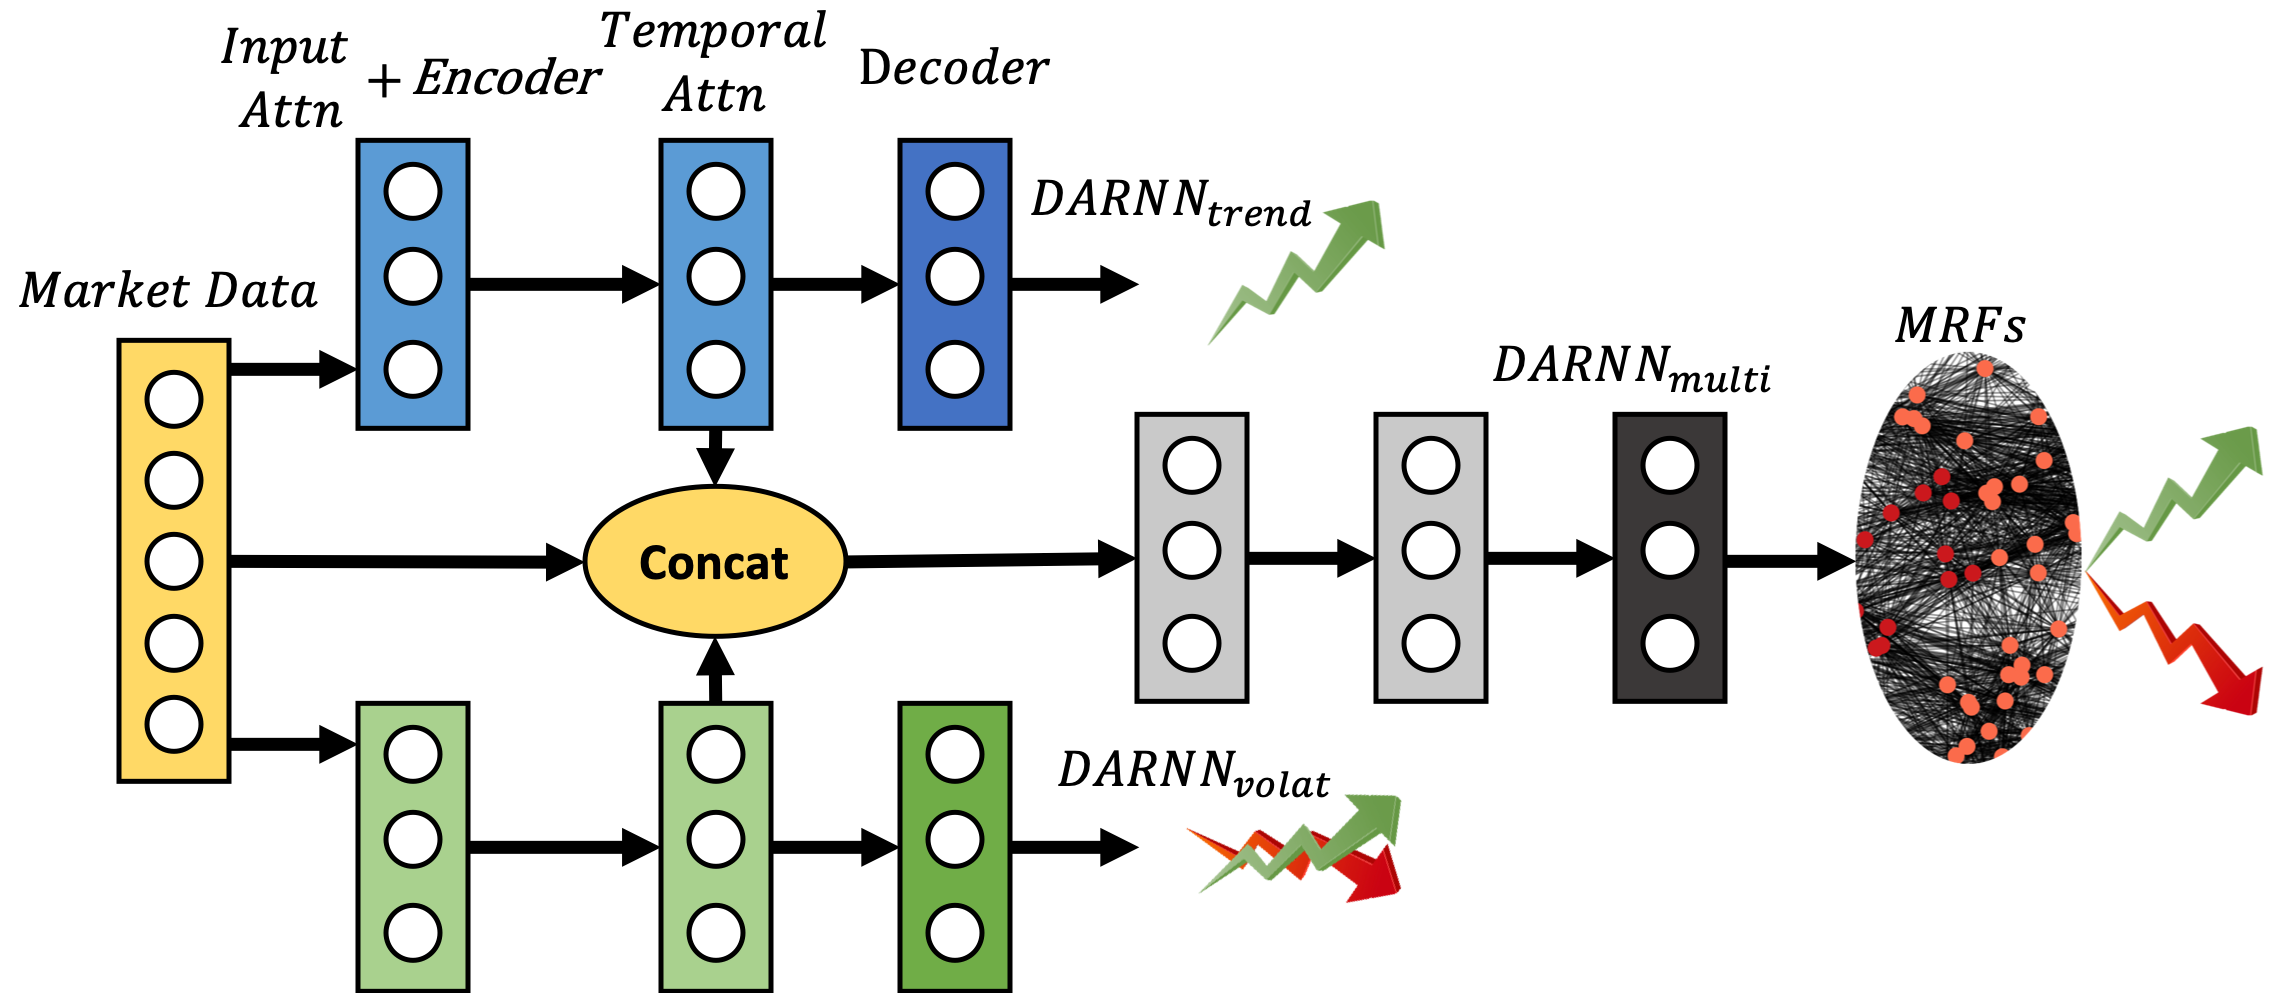
\includegraphics[width=1\columnwidth]{Methodology/figures/mmplmrf.png}
  \caption{\label{fig:mrfrnn} Multi-task RNN-MRFs architecture. Note 
  that the output of $\text{DARNN}_{\text{multi}}$ only corresponds to one 
  node's unary feature in MRFs.}\vspace{-5mm}
\end{figure}

All three DARNN modules share the same raw market price data.
Here, we denote the time-series dataset as $\bX$ where
$\bX=(\bx_1,\bx_2,\dots,\bx_T)\in \reals^{N\times T}$. We use
$\bx^n=(x_1^n,x_2^n,\dots,x_T^n) \in \reals^T$ to denote a driving
series of $T$ time-steps and $\bx_t=(x_t^1,x_t^2 ,\dots
,x_t^N)\in \reals^N$ to denote a snapshot at time-step $t$ of all
$N$ features.

For both DARNN modules at the low level, the input is $\bX \in \reals^{5\times T}$
which contains $5$ exogenous driving series, \textit{i.e.}, opening price, low
price, high price, volume, amount and $1$ target series $\by =
(y_1,y_2,\dots,y_T) \in \reals^T$. These two modules
aim to predict target series $y_{t+p}$ in the next $p$ time
steps:

$$\hat{y}_{t+p} = \text{DARNN}(y_1,\dots,y_{t},x_1,\dots,x_t)$$

The target series $\by_{\text{trend}}$ of
$\text{DARNN}_{\text{trend}}$ is the closing price. The target series
$\by_{\text{volat}}$ of $\text{DARNN}_{\text{volat}}$ is the
standard deviation of closing price over $M$ constant time-steps.
In our implementation we set $M=10$. We use Mean Squared Error
(MSE) as the loss function to train those two modules separately.

To construct the high level DARNN module, which aims to predict
the price movement, we concatenate context vectors $\bc_T$ from
each of low level DARNN module's encoder and raw market price
matrix as the input. The target series $\by^{\text{binary}}$ is
constructed by the sign function $y_t^{\text{binary}} =
sign(y_{t+p}-y_t)$ where $y_t$ denotes closing price at time-step
$t$. We use cross-entropy as loss function to train the final
$\text{DARNN}_{\text{multi}}$. Logits (outputs before going
through \emph{softmax}) of $\text{DARNN}_{\text{multi}}$ are then
passed to Intra-clique Predictor as unary features.

In order to train MMPL together with MRFs in an end-to-end
manner, we follow the subgradient method proposed by
\citename{witoonchart2017application}. Since our inner loop
proposed in section~\ref{sec:mrflssvm_learning_algo} is actually
a latent structural SVM. Only gradients of parameters and feature
functions need to be updated. In our framework, outputs of
MMPL (Logits of $\text{DARNN}_{\text{multi}}$) are only used as unary features in MRFs' energy functions,
our back-propagation rules can be defined by taking derivative of the objective function defined in
~\eqref{eq:mrflssvm_object}:

\begin{align}
  \label{eq:der_w}
  \frac{\partial L}{\partial \bw^U} = \psi^U(y)-\psi^U(y^*)
\end{align}

\noindent where $y$ is the ground-truth label and $y^*$ is
inferenced label. $\psi^U$ is unary feature
function described in section~\ref{sec:llep}, here it denotes
logits calculated from $\text{DARNN}_{\text{multi}}$. $\bw^U$ is
unary parameter defined in energy function~\eqref{eq:energyfunction_UPH}.
Equations \eqref{eq:der_w} can be directly plugged
into sub-gradient algorithm proposed in \cite{witoonchart2017application}.
Other configurations stay the same with their algorithm.

\subsection{Intra-clique Predictor}
\label{sec:srp}

In this section, we show how to construct an ``Intra-clique
Predictor" to model lead-lag relationships and address the other
two challenges as mentioned in the introduction. Specifically, we
present a binary Markov Random Fields (MRFs) with weighted lower
linear envelopes as higher order (when the clique contains more
than two nodes) energy functions. Note that the algorithm
proposed here is a general framework for classification tasks.
Besides time series classification, it can also be applied to other tasks such as computer vision.

% In section~\ref{sec:opt} we will discuss learning the
% parameters under the latent structural SVM framework and also
% how to back-prop gradients to neural networks.


\subsubsection{Higer Order Energy: The Weighted Lower Linear
  Envelope Function}
\label{sec:llep}

Energy functions can be decomposed over nodes $\N$, edges $\E$
and higher order cliques $\cal C$~\cite{Szummer:ECCV08}. Let
$\bw$ be vector of parameters and $\psi$ be arbitrary feature
function, then the energy can be decomposed as a set of linear
combinations of weights and feature vectors:

\begin{align}
  \label{eq:energyfunction_UPH}
  E(\by;\bw)&=\sum_{i\in \N}{\bw_i^U\psi^U(\by_i)}+ \notag\\
  & \sum_{(i,j)\in \E}{\bw_{ij}^P\psi^P(\by_i,\by_j)}+
  \sum_{\by_C\in \cal C}{\bw_C^H\psi^H(\by_C)}
\end{align}

\noindent where $U$ denotes \emph{unary} terms, $P$ denotes
\emph{pairwise} terms, $H$ denotes \emph{higher order} terms.
In this section we mainly focus on one class of higher-order
potentials $\psi^H$ defined as a concave piecewise linear
function which is known as \emph{lower linear envelope
  potentials}. This has been studied extensively in Markov Random
Fields area for encouraging consistency over large
cliques~\cite{Kohli:CVPR07,Nowozin:2011,Gould:ICML2011}.

Let $\cal C$ denotes the set of all maximal cliques
and $\by_c=\{y_i |\text{\,for\,} i \in C_j\}$ denotes set of
binary random variables where $y_i\in \{0,1\}$ in clique $C_j$, a
weighted lower linear envelope potential over $\by_c$ is defined
as the minimum over a set of $K$ linear functions as:
%
\begin{align}
  \psi^H_c\!(\by_c) \, &= \min_{k=1, \ldots, K} \left\{ a_k W_{\!c}(\by_c) + b_k \right\}.
  \label{eqn:potential2}
\end{align}
%
where $W_{\!c}(\by_c) = \sum_{i \in c} w_i y_i$ with $w^c_i \geq
0$ and $\sum_{i \in c} w^c_i = 1$ which are weights for each
clique. $(a_k, b_k) \in \reals^2$ are the linear function
parameters. We illustrate an example with
four linear functions in \figref{fig:concave}.

\begin{figure}[t]
  \centering
  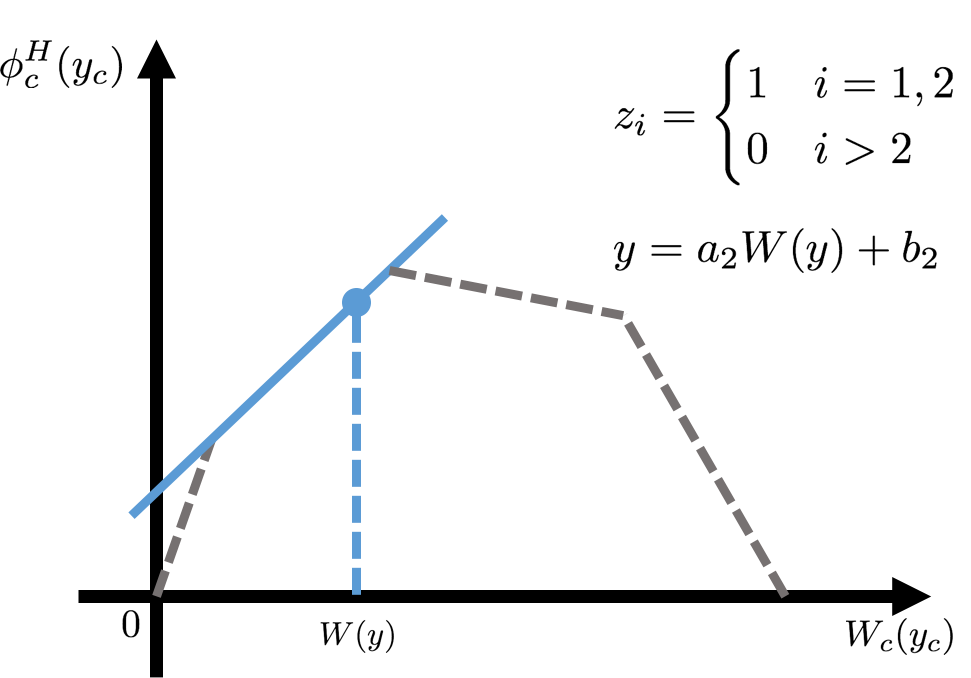
\includegraphics[width=0.8\columnwidth]{Methodology/figures/linEnvLatentFig.png}
  \caption{\label{fig:concave} Example piecewise-linear concave
    function of $W_{\!c}(\by_c) = \sum_{i \in c} w^c_i y_i$.
    Assume the second linear function is active namely
    $\bz^c=(1,1,0,0)$ (equation \ref{eqn:binary_concave_z}). The result of linear combination of
    parameter vector and feature vector is same as quadratic
    psuedo-Boolean function.}
\end{figure}

% % to_replace
% \begin{figure}[ht]
%   \centering
%   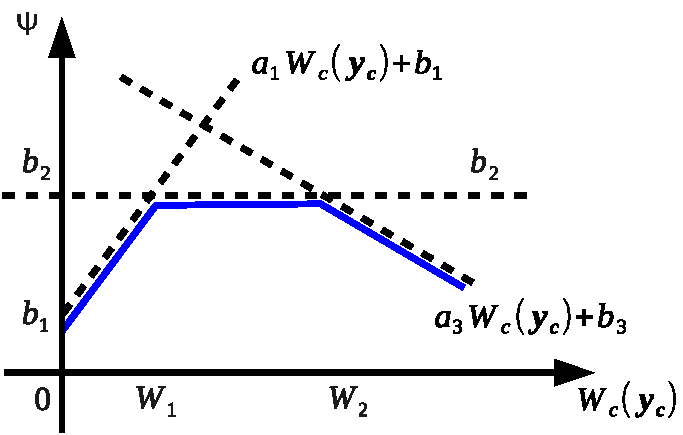
\includegraphics[width=0.6\columnwidth]{Methodology/figures/not_redundant}
%   \caption{\label{fig:nonredundant} Example lower linear envelope
%     $\psi^H_c\!(\by_c)$ (shown solid) with three terms (dashed).
%     When $W_{\!c}(\by_c) \leq W_1$ the first linear function is
%     active, when $W_1 < W_{\!c}(\by_c) \leq W_2$ the second
%     linear function is active, otherwise the third linear
%     function is active.}
% \end{figure}

Inference on energy function contains lower linear potentials is
the same as the standard equation~\eqref{eq:energyfunction_UPH}
and is given by:
\begin{align}
  \label{eq:min_energy}
  \by^* = \argmin\energy{\by}
\end{align}

To ensure potentials do not contain redundant linear functions
(functions that would never be active), \citename{gouldlearning}
proposed a constraint on parameters of the envelope. The $k$-th
linear function is not redundant if the following condition is
satisfied:
%
\begin{align}
    0
    <
    \frac{b_k - b_{k-1}}{a_{k-1} - a_k}
    <
    \frac{b_{k+1} - b_k}{a_k - a_{k+1}}
    <
    1.
  \label{eq:nonredundant}
\end{align}
%
Another important property of equation~\eqref{eq:min_energy} is
shift invariant (vertically). We write
$\widetilde{\psi}^{H}_c\!(\by_c)$ by shift
equation~\eqref{eqn:potential2} vertically with an abitrary
amount $b^{const}\in R$
$$\widetilde{\psi}^{H}_c\!(\by_c) = \min_{k=1, \ldots, K}
\left\{a_k W_{\!c}(\by_c) + b_k + b^\textrm{const} \right\}$$
%
Then we have
\begin{align}
  \argmin_{\by_c} \psi^H_c\!(\by_c)
  = \argmin_{\by_c} \widetilde{\psi}^{H}_c\!(\by_c).
  \label{eq:shift_invariant}
\end{align}
%
Therefore, in the following discussion without loss of generality
we assume $b_1 = 0$ thus $b_k\geq0 \text{\; for \;} k=1,\dots,n$.
%
\subsubsection{Exact Inference}
\label{sec:exact_inference}

Exact inference on MRFs has been extensively studied in past
years. Researchers found that, energy functions which can be
transformed into quadratic pseudo-Boolean
functions~\cite{Ishikawa:PAMI03,Ishikawa:CVPR09,Rother:CVPR09}
are able to be minimized exactly using \emph{graph-cuts} like
algorithms~\cite{Freedman:CVPR05,Hammer:1965} when they satisfy
submodularity condition~\cite{Boros:MATH02}.
\citename{Kohli:TR08} and \citename{Gould:ICML2011} adapted those
results to perform exact inference on lower linear envelope
potentials. In this section we mainly focus on describing the
\emph{st min cut} graph constructed by
Gould~\cite{Gould:ICML2011,gouldlearning} for exact
inference~\eqref{eq:min_energy} of energy function containing
lower linear envelope potentials.

Following the approach of \citename{Kohli:CVPR10},
\citename{Gould:ICML2011,gouldlearning} transformed the weighted
lower linear envelope potential~\eqref{eqn:potential2} into a
quadratic pseudo-Boolean function by introducing $K-1$ auxiliary
variables $\bz = \left(z_1, \ldots, z_{K-1}\right)$ with $z_k\in
\{0,1\}$:

\begin{align}
  E^c(\by_c, \bz) &= a_1 W_{\!c}(\by_c) + b_1 \notag \\
  &+ \sum_{k = 1}^{K-1} z_k \left( \left(a_{k+1} - a_k\right) W_{\!c}(\by_c) + b_{k+1} - b_k \right)
  \label{eqn:binary_concave_z}
\end{align}

\noindent for a single clique $c \in \cal C$. Under this formulation,
minimizing the pseudo-Boolean function over $\bz$ is equivalent
to selecting (one of) the active functions(s) from
equation~\eqref{eqn:potential2}. Another important property of
optimized $\bz$ under this formulation is that it automatically
satisfies the constraint: $z_{k+1} \leq z_k$. This property give rise to further development of
parameter vector and feature
vector (equation~\eqref{eq:llsvm_param} and ~\eqref{eq:llsvm_feature})
which are used in latent
structural SVM.

\begin{figure}[t]
  \centering
  \setlength{\tabcolsep}{2pt}
  \begin{tabular}{cc}
    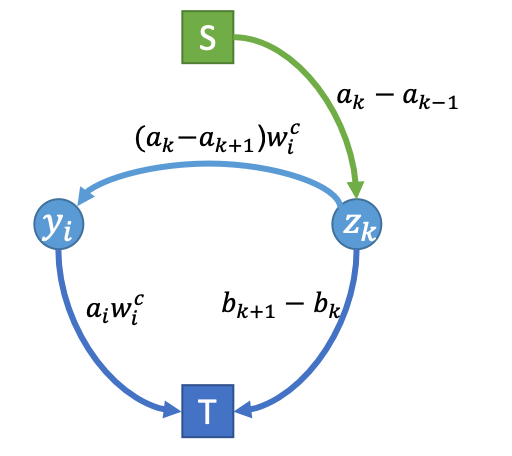
\includegraphics[width=0.54\columnwidth]{Methodology/figures/ho.png}&
                                                                         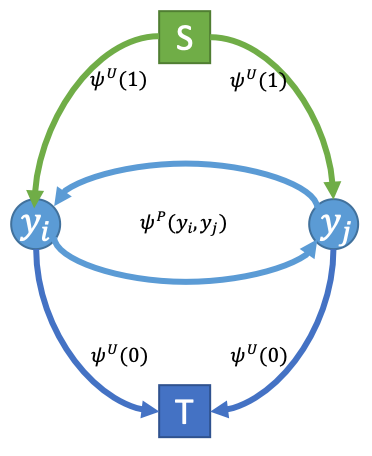
\includegraphics[width=0.4\columnwidth]{Methodology/figures/up.png}\\
                                                                         {\small (a)} & {\small (b)} 
  \end{tabular}
  \caption{\label{fig:stmincut} $st$-graph construction for
    equation~\eqref{eqn:posiform}, unary and pairwise terms.
    Every cut corresponds to an assignment to the random
    variables, where variables associated with nodes in the
    ${\cal S}$ set take the value one, and those associated with
    nodes in the $\T$ set take the value zero. With slight abuse
    of notation, we use the variables to denote nodes in our
    graph.}
\end{figure}



In order to construct the \emph{st-min-cut} graph, we rewrote
equation~\eqref{eqn:binary_concave_z} into
\emph{posiform}~\cite{Boros:MATH02}:

\begin{align}
  \label{eqn:posiform}  
  E^c(\by_c, \bz)
  &= b_1 - (a_1 - a_K) + \sum_{i \in c} a_1 w^c_i y_i \notag\\
  & + \sum_{k = 1}^{K - 1} \left( b_{k+1} - b_k \right) z_k
    + \sum_{k = 1}^{K - 1} \left( a_k - a_{k+1} \right)
    \bar{z}_k\notag\\
  & + \sum_{k = 1}^{K - 1} \sum_{i \in c} \left( a_k - a_{k+1}
    \right) w^c_i \bar{y}_i z_k
\end{align}

\noindent where $\bar{z}_k = 1 - z_k$ and $\bar{y}_i = 1 - y_i$.
$a_1$ is assumed to be greater than $0$ so that all coefficients
are positive (recall we assume $b_1=0$ in section~\ref{sec:llep}
and we have $a_k > a_{k+1}$ and $b_k < b_{k+1}$). Since the energy function~\eqref{eqn:posiform}
is submodular, the \emph{st-min-cut} graph can be constructed 
based on equation~\eqref{eqn:posiform}. The construction (including 
unary and pairwise) is explained in \figref{fig:stmincut}. 

% Figure
% (a) denotes construction for equation~\eqref{eqn:posiform}. For
% each lower linear envelope potential edges are added as follows:
% for each $i \in c$, add an edge from $y_i$ to $t$ with weight
% $a_1 w^c_i$; for each $i \in c$ and $k = 1, \ldots, K-1$, add an
% edge from $z_k$ to $y_i$ with weight $(a_{k} - a_{k+1}) w^c_i$;
% and for $k = 1, \ldots, K-1$, add an edge from $s$ to $z_k$ with
% weight $a_k - a_{k+1}$ and edge from $z_k$ to $t$ with weight
% $b_{k+1} - b_k$. Figure (b) denotes construction for unary and
% pairwise terms (see \cite{Kolmogorov:PAMI04}). For unary edges (4
% edges on both sides), weights on each edge are corresponding to
% values in input unary terms accordingly. For pairwise edges (2
% edges in the middle), both edges share the same weight which
% equals to the input pairwise term.

\section{Optimization}
\label{sec:opt}

\subsection{Transforming Between Representations}
\label{sec:learning}
With the inference algorithm in hand, we now can develop the
learning algorithm for weighted lower linear envelope potentials
using the latent structural SVM framework. We begin by
transforming the equation~\eqref{eqn:binary_concave_z} into a
linear combination of parameter vector and feature vector. Then a
two-step algorithm was developed to solve the latent structural
SVM.

The latent structural SVM formulation requires that the energy
function be formulated into a linear combination of features and
weights while our higher-order potential is represented as the
minimum over a set of linear functions. However,
in~\ref{sec:exact_inference} we reformulated the piesewise linear
functions into a quadratic pseudo-Boolean
function~\eqref{eqn:binary_concave_z} by introducing auxiliary
variables. Now we show function~\eqref{eqn:binary_concave_z}
itself is an inner product of parameter vector and feature vector
with latent information. Note that the function can be expanded
as a summation of $2K-1$ terms:

\begin{align}
  \label{eq:originalenergy}
  E^c(y_c,z)
  =&a_1W_c(y_c)+\sum_{k=1}^{K-1}(a_{k+1}-a_k)z_kW_c(y_c) \notag \\
   &+\sum_{k=1}^{K-1}(b_{k+1}-b_k)z_k
\end{align}

Here we use the fact of equation~\eqref{eq:shift_invariant} and
let $b_1=0$. Now we can reparameterize the energy function
as
\begin{align}
  \label{eq:llsvm_innerprod_energy}
  E^c(\by_c,\bz; \btheta) = \btheta^T \! \psi(\by_c,\bz)
\end{align}

\noindent where:

\begin{equation}
\label{eq:llsvm_param}
  \theta_k = \left\{
    \begin{aligned}
      & a_1	& \text{for} \ k=1\\
      & a_k-a_{k-1} & \text{for}\ 1< k \leq K\\
      & b_{k+1-K}-b_{k-K} & \text{for} \ K<k\le2K-1\\
    \end{aligned}
  \right.
\end{equation}

\begin{equation}
\label{eq:llsvm_feature}
  \psi_k = \left\{
		\begin{aligned}
      & W_c(\by_c) 	& \text{for} \ k=1\\
      & W_c(\by_c)\bz_k & \text{for}\ 1<k\le K\\
      & \bz_k & \text{for} \ K<k\le2K-1\\
		\end{aligned}
  \right.
\end{equation}

Under this formulation, inference problems in
\cite{yu2009learning} can be written as:

\begin{align}
  \label{eq:linenv_full_inf}
  (\mathbf{\hat{y}}_k(\btheta),\mathbf{\hat{z}}_k(\theta))=\argmin_{(\mathbf{y}
  \times \mathbf{z}) \in \mathcal{Y} \times \mathcal{Z}}
  \btheta^T\cdot\psi(\mathbf{y}_k,\mathbf{z}_k)
\end{align}
and
\begin{align}
  \label{eq:linenv_latent_inf}
  \mathbf{z}^*_k(\btheta) = \argmin_{\mathbf{z} \in \mathcal{Z}}
  \btheta^T \cdot \psi(\mathbf{y}_k,\mathbf{z}_k)
\end{align}

There are 2 facts worth to mention. The first fact is
that in our previous construction of minimum-$st$-cut graph the
latent variable $\bz$ is already included. Therefore, we can
apply our inference algorithm directly on our 2 new formulations.

More interesting for equation~\eqref{eq:linenv_latent_inf} there exists
more efficient algorithm. At training stage the ground-truth
labels $y_i$ is a function input thus completely observed.
Therefore, the term $((a_{k+1}-a_k)W_c(\by_c)+b_{k+1}-b_k)$ in
equation~\eqref{eq:originalenergy} becomes constant. So we can
infer latent variable $\bz$ explicitly by:
\begin{align}
  \label{eq:linenv_effi_infer_latent}
  z_k^c &=
          \begin{cases}
            0 & \text{if $((a_{k+1}-a_k)W_c(y_c)+b_{k+1}-b_k)\geq0$} \\
            1 & \text{otherwise}.
          \end{cases}
\end{align}

Therefore, assignments inferred by graph-cut algorithm can be
directly encoded into a linear combination by using our latent
structural SVM formulation for learning purpose. The remaining
task is to ensure the concavity of $\btheta$. We do this by
adding following constraint:

\begin{align}
  \label{eq:concave_constraint}
  A\btheta\geq\epsilon \text{,\;~~~} A=
                  \begin{bmatrix}
                    1 & \mathbf{0} & \mathbf{0}\\
                    \mathbf{0} & -\mathbf{1} & \mathbf{0}\\
                    \mathbf{0} & \mathbf{0} & \mathbf{P}
                  \end{bmatrix}\in \mathbb{R}^{(2K-1)\times(2K-1)}
\end{align}

\noindent where $-\mathbf{1}$ is a matrix of size $(K-1)\times(K-1)$ and
$\mathbf{P}$ is an identity matrix of size $(K-1)\times(K-1)$.
One subtle problem we found during experiments is that the
algorithm can be stuck with small numerical value. To avoid this
we add small slack variables $\epsilon=\mathbf{1}^{-15}$ on 
those constraints.

\subsection{Latent Structural SVM Learning}
\label{sec:mrflssvm_learning_algo}

With the inner product formulation
(equation~\eqref{eq:llsvm_innerprod_energy}) of higher order
energy function in hand, we now able to develop our latent
structural SVM learning algorithm. The energy function (higher
order function together with unary and pairwise functions) can be
written as:
\begin{equation}
  E_{all}(y,z) = \begin{bmatrix}
    \btheta^H\\
    \theta^{unary}\\
    \theta^{pairwise}
  \end{bmatrix}^T 
  \cdot \begin{bmatrix}
    \psi^H\\
    \psi^{unary}\\
    \psi^{pairwise}
  \end{bmatrix}=\theta_{all}^T\cdot\psi_{all}
\end{equation}
where $\btheta^H\in \reals$ is the parameter vector in higher
order equation~\eqref{eq:llsvm_innerprod_energy} of size $2K-1$.
$\theta^{unary}$ and $\theta^{pairwise}$ are both scalars.
$\psi^\textrm{unary} = \sum_i \psi^U_i\!(y_i)$ and
$\psi^\textrm{pairwise} = \sum_{ij} \psi^P_{ij}(y_i, y_j)$.
Therefore, the size of $\theta_{all}$ is $2K+1$.

% Plug equation~\eqref{eq:linenv_full_inf} and
% equation~\eqref{eq:linenv_latent_inf} into object function in
% \cite{yu2009learning}, the latent structural SVM object function
% for our problem can be derived as a difference of two convex
% functions:

% \begin{align}
% \label{eq:lssvm_object}
%   \min_\theta\bigg(\frac{1}{2}\|\theta\|^2+
%   C\sum_{i=1}^{n}\big(\max_{(\mathbf{\hat{y}} \times
%   \mathbf{\hat{z}}) \in \mathcal{Y} \times \mathcal{Z}}
%   [\theta\cdot\psi(\mathbf{\hat{y}},\mathbf{\hat{z}}) +
%   \Delta(\mathbf{y}_i,\mathbf{\hat{y}},\mathbf{\hat{z}})]\big)\bigg)\\
%   -C\sum_{i=1}^{n}\big(\max_{\mathbf{z} \in \mathcal{Z}} \theta \cdot
%   \psi(\mathbf{y}_i,\mathbf{z})\big)\nonumber
% \end{align}

Following \citename{yu2009learning}, we use the two stages Concave-Convex
Procedure (CCCP)~\cite{yuille2002concave} to solve the
optimization problem. We first
imputes the latent variables $\bz$ explicitly by
equation~\eqref{eq:linenv_latent_inf}. Namely solving the
``latent variable completion'' problem~\cite{yu2009learning}:

% \begin{align}
%   \bz_i^*=\argmax_{\mathbf{z} \in \mathcal{Z}} \theta \cdot
%   \psi(\mathbf{y}_i,\mathbf{z})
% \end{align}

The inference result $z_i^*$ for $i=1,\dots,n$ is used as
completely observed for later stage. With the latent variable
$z_i^*$ which best explains the ground-truth data $y_i$ in hand,
updating the parameter vector $\btheta$ reduces to solve the
standard structural SVM problem:

\begin{align}
\label{eq:mrflssvm_object}
  \min_\theta\bigg(\frac{1}{2}\|\theta\|^2+
  C\sum_{i=1}^{n}\big(\max_{(\mathbf{\hat{y}} \times
  \mathbf{\hat{z}}) \in \mathcal{Y} \times \mathcal{Z}}
  [\theta\cdot\psi(\mathbf{\hat{y}},\mathbf{\hat{z}}) +
  \Delta(\mathbf{y}_i,\mathbf{\hat{y}},\mathbf{\hat{z}})]\big)\bigg)\\
  -C\sum_{i=1}^{n}\big(\theta \cdot
  \psi(\mathbf{y}_i,\mathbf{z}_i^*)\big) \nonumber
\end{align}

Our optimization algorithm is summarized in
\algref{alg:learning}. As we mentioned in
\appref{sec:train_detail}, although we proposed an end-to-end
subgradient algorithm is section \ref{sec:mmpl}, MRFs updated by
such algorithm take too many iterations to converge. Therefore,
we propose a two-stage training procedure. At first stage, MMPL
and MRFs are trained separately. Therefore, MRFs can take
advantage of the efficient latent structural SVM and converge in
a polynomial number of iterations. After all those models are
converged, we then combine them together to conduct end-to-end
training. Note that the CCCP Inner Loop in \algref{alg:learning}
is actually solving standard structural SVM problem. Therefore,
at the second stage, we use subgradient algorithm proposed in
section~\ref{sec:mmpl} to replace the CCCP Inner Loop. Other
settings remain the same.

The last problem remaining is the initialization method. Because
our objective function~\eqref{eq:mrflssvm_object} is not convex
and the CCCP algorithm is only guaranteed to converge to a local
minimum or saddle point\cite{yuille2002concave}, initialization
of $\btheta$ might affect the performance of our algorithm. Since
there are no theoretical solution for this problem, we propose an
empirical initialization algorithm in \appref{sec:sup_init}.

\section{Experiment}
\label{sec:exp}

In this section, we first introduce 3 stock datasets. Then, we
introduce the parameter settings for our model and training
details. Finally, we select four evaluation metrics and use them
to demonstrate the effectiveness of our proposed model by comparing to
several baseline approaches.

\subsection{Dataset and Model Settings}
\label{sec:dataset}

To demonstrate the effectiveness of higher order consistency, we
choose three exclusive and the most famous stock indexes on Chinese
stock market to build our input datasets. Their index codes are:
CSI (China Securities Index) 200, CSI 300 and CSI 500 which
contain 200, 500 and 300 constituent stocks respectively. The CSI
300 index selects most liquid A-share stocks. It aims to reflect
the overall performance of China A-share market. The CSI 200 and
500 indexes aim to reflect the overall performance of mid-to-large
and small-to-mid capital A-shares respectively.

All these indexes are exclusive and are refined on a yearly
basis. In this paper, we use fixed versions on 30-JAN-2015. We
then collect their constituent stocks' minute-level data from
05-JAN-2015 to 29-DEC-2017. On Chinese stock market each trading
day has 4 trading hours. So there are 240 samples (minutes) for
each normally traded stock on each day. Each sample contains 6
features: opening price, high price, low price, closing price,
volume, and amount. \footnote{During this period, there are some
  stocks de-listed (SZ000024, SH600485, SH600832 in CSI 200;
  SZ000693, SZ000748, SZ000982 in CSI 500; SH600485, SH600832,
  SZ000024, SH601299 in CSI 300). Therefore, in total we collect
  197, 497 and 296 stocks during this period respectively.} For
each stock, the first $80\%$ days are used to construct the
training set and the last $20\%$ days are used as test set.
Approximately training set and test set contain $33.6$ million
and $4.2$ million samples, respectively. $49.5\%$ of them are
positive movements, $0.3\%$ of them stay unchanged and $50.2\%$
of them are negative movements. For binary classification task,
we follow \citename{mitchell2001characteristics}'s approach and
label all positive movement samples $1$ and $0$ for the other
samples. More labeling details are described in appendix
\ref{sec:train_detail}.

\begin{table}[H]
\centering
\small
\caption{Technical Indicators Selection}
\begin{tabular}{|c|c|} \hline
  Category&Indicator Name\\ \hline
  Momentum& Awesome Oscillator, Money Flow Index\\ \hline
  Volume& \makecell{Chaikin Money Flow\\ On-balance volume mean}\\ \hline
  Volatility& Bollinger Bands (Upper and Lower Bands)\\ \hline
  Trend& \makecell{Average Directional Movement Index\\Moving Average Convergence Divergence}\\ \hline
\end{tabular}
  \label{tab:ta}
\end{table}
\vspace{-2mm}
To demonstrate the benefits of multi-task RNN over manually designed
technical indicators, we construct technical
indicators datasets. We select 8 most popular indicators, 2 from each
category~\cite{kirkpatrick2010technical} shown in Table
\ref{tab:ta}. In implementation, we use open source package
\emph{Technical Analysis Library in
  Python\footnote{https://github.com/bukosabino/ta}} to calculate
those indicators and all hyperparameters are using package's
default settings without any prior expert knowledge involved
with. After technical indicators calculation, these 8 new
features are concatenated to above market price dataset (5
features at each minute). So the final input dataset for each
single task model contains 13 features in total. Before feeding
into models, we normalize each stock with \emph{z-score} function
using standard deviation and mean calculated in the training set.

For brevity, we denote market price dataset which only contains
$5$ features as \textbf{Market} and the concatenated $13$
features dataset as \textbf{Indicator}. As discussed in
section~\ref{sec:mmpl}, closing price at time $t$ can be directly
used as regression target for $\text{DARNN}_{\text{trend}}$.
Standard deviation of closing price with a window size of $10$ is
used as regression target for $\text{DARNN}_{\text{volat}}$. The
dimensions of hidden state and cell state are fixed as 32 for
$\text{DARNN}_{\text{trend}}$ as well as
$\text{DARNN}_{\text{volat}}$, and 128 for
$\text{DARNN}_{\text{multi}}$. More training details are
described in appendix \ref{sec:train_detail}.

\subsection{Results}
\label{sec:res}

In order to demonstrate the effectiveness of our framework, we
compare 3 baseline methods, \textit{i.e.},
LSTM~\cite{hochreiter1997long}, attention based LSTM
Encoder\_Decoder~\cite{attention}, and DARNN~\cite{qin2017dual}
on 3 different Chinese Securities Indexes with and without
technical analysis indicators as inputs. Results are summarized
in Table~\ref{tab:result}. All results are reported over the test
sets. We select four metrics (Accuracy, Precision, Recall and F1
Score) as evaluation metrics to justify the effectiveness of the
proposed approach. They are calculated by collecting all
predicted labels of constituent stocks in each CSI index.


\begin{table*}[t]
\centering
\small
\setlength\tabcolsep{2pt}
\caption{Results: Baselines and ablation study. All models have a
  window size (lag steps) of 20 and predict price movement label
  at the next time step.}
\begin{tabular}{@{}cccccccccccccc@{}}
\toprule
Data Set                   & Models                          & \multicolumn{12}{c}{Chinese Securities Index (CSI)}                                                                                                                                                                                                    \\ \midrule
\multicolumn{2}{c}{\multirow{2}{*}{}}                        & \multicolumn{4}{c}{CSI200}                                                                & \multicolumn{4}{c}{CSI500}                                                             & \multicolumn{4}{c}{CSI300}                                        \\
\multicolumn{2}{c}{}                                         & Accuracy                   & Precision      & Recall         & F1 Score                   & Accuracy       & Precision      & Recall         & F1 Score                            & Accuracy       & Precision      & Recall         & F1 Score       \\ \cmidrule(r){1-2} \cmidrule(lr){4-5} \cmidrule(lr){8-9} \cmidrule(lr){12-13}
\multirow{3}{*}{\textbf{Indicator}} & LSTM                            & 62.30                      & 73.82          & 70.70          & 72.23                      & 60.35          & 68.56          & 70.03          & 69.29                               & 60.16          & 71.39          & 68.50          & 69.91          \\
                           & \multicolumn{1}{c|}{LSTM Encoder\_Decoder} & 64.26                      & 72.41          & \textbf{74.34} & \multicolumn{1}{c|}{73.36} & 61.13          & 75.63          & 66.67          & \multicolumn{1}{c|}{70.86}          & 64.26          & 75.54          & 70.57          & 72.97          \\
                           & DARNN                           & 63.09 & 72.08          & 73.55          & 72.81                      & 66.60          & 78.98          & \textbf{74.13}          & \textbf{76.48}                               & 65.82          & 76.68          & 73.46          & 75.04          \\ \cmidrule(r){1-2} \cmidrule(lr){4-5} \cmidrule(lr){8-9} \cmidrule(lr){12-13}
\multirow{5}{*}{\textbf{Market}}    & LSTM                            & 57.62                      & 67.57          & 67.37          & 67.47                      & 55.86          & 68.10          & 64.53          & 66.27                               & 56.25          & 67.17          & 65.98          & 66.57          \\
                           & \multicolumn{1}{c|}{LSTM Encoder\_Decoder} & 59.57                      & 71.60          & 66.86          & \multicolumn{1}{c|}{69.15} & 58.40          & 69.53          & 68.12          & \multicolumn{1}{c|}{68.81}          & 61.33          & 71.87          & 68.91          & 70.36          \\
                           & \multicolumn{1}{c|}{DARNN}      & 61.13                      & 71.26          & 71.47          & \multicolumn{1}{c|}{71.37} & 63.09          & 77.04          & 67.87          & \multicolumn{1}{c|}{72.16}          & 63.87          & 72.09          & 73.59          & 72.83          \\
                                                      & \multicolumn{1}{c|}{$\text{DARNN}_\text{trend}+\text{DARNN}_\text{multi}$}      & 63.67 & 74.77 & 71.38 & \multicolumn{1}{c|}{73.04} & 62.89          & 75.30          & 69.38          & \multicolumn{1}{c|}{72.22}          & 62.69          & 73.84          & 66.56          & 70.00          \\
                           & \multicolumn{1}{c|}{$\text{DARNN}_\text{volat}+\text{DARNN}_\text{multi}$}      & 62.50                      & 73.97          & 71.06          & \multicolumn{1}{c|}{72.49} & 62.30          & 74.46          & 69.20          & \multicolumn{1}{c|}{71.74}          & 61.91          & 72.98          & 68.51          & 70.67          \\

                           & \multicolumn{1}{c|}{MMPL}       & 65.04                      & 74.04          & 73.39          & \multicolumn{1}{c|}{73.72} & 65.43          & 76.04          & 72.80 & \multicolumn{1}{c|}{74.38} & 66.60          & 71.67          & \textbf{78.90} & 75.11          \\
                           & MMPL+MRFs                       & \textbf{67.97}             & \textbf{77.51} & 73.91          & \textbf{75.67}             & \textbf{66.80} & \textbf{79.65} & 72.78          & 76.06                               & \textbf{68.95} & \textbf{78.55} & 74.71          & \textbf{76.58} \\ \bottomrule
\end{tabular}
\label{tab:result}
\end{table*}

\subsubsection{Effectiveness of multi-task framework}

As mentioned earlier, to demonstrate effectiveness of multi-task
framework, we use \textbf{Indicator} dataset, which contains both
market price data and technical analysis indicators as inputs for
baseline approaches and \textbf{Market} dataset which only
contains market price data as inputs for MMPL (multi-task RNN) as
well as baseline methods. For DARNN, we use a hidden size of
$128$. MMPL's configuration is described in
section~\ref{sec:multi_train}. As we can see in
Table~\ref{tab:result}, single task models (LSTM, LSTM
Encoder\_Decoder, DARNN) tested on \textbf{Market} dataset
(without technical analysis indicators as inputs) generally have
worse performance with all 4 metrics. In particular, performance of
DARNN models tested on \textbf{Indicator} dataset is consistently
better than the ones on \textbf{Market} dataset. This proves that
even with hand-crafted features, deep learning models can still
benefit from diversified and complementary features.

To test the effectiveness of multi-task framework, we conduct ablation study with only one low-level task (\quad $\text{DARNN}_\text{trend}$ \quad or \\ $\text{DARNN}_\text{volat}$) 
together with the high-level task module $\text{DARNN}_\text{multi}$. Results
indicate that these two variants have comparable or slightly worse result than
 DARNN on \textbf{Market}. This may because single task model does not provide diversified features while have more parameters than DARNN. Finally, MMPL outperforms all single task models and baseline methods on \textbf{Market}. This
suggests that diversified and complementary tasks can help MMPL extract effective features. Specifically,
by comparing MMPL and DARNN on \textbf{Market} as well as \textbf{Indicator},
we can see that MMPL generally outperforms DARNN on CSI200 and
CSI300 indexes and is slightly worse than DARNN on \textbf{Indicator} of CSI500 index. We can conclude that by using multi-task
RNNs, we can extract better or at least comparable features compared with
hand-crafted features.
\subsubsection{Effectiveness of higher-order MRFs}
In Table~\ref{tab:result}, we can observe that MMPL-MRFs framework consistently outperforms other baselines on all 3 CSI index constituent stocks. It shows evidence that higher-order energy function can help with
encoding clique level consistency thus improving overall
prediction performance. One interesting point to note is that the recall rate of MMPL-MRFs is constantly lower than other baselines. This can be seen as a trade off between accuracy and recall rate. However, it is worth to mention that for stock price movement prediction, high accuracy and precision are much preferred than recall rate. Another interesting phenomenon is that MMPL-MRFs gives higher improvements on CSI200 and CSI300 while little improvements over DARNN trained with technical
analysis indicators on CSI500. One possible reason is that CSI200 and CSI300 select most liquid and representative stocks in Chinese stock market. Those stocks exhibit much stronger and higher order consistency than illiquid stocks. CSI500 selects small-mid
capital stocks which are less liquid and contains much more noisy movements.

During training time, our algorithm converges in from 4 to 19
CCCP outer loops. The average inference time of graph-cut
algorithm is 34 seconds.

\subsubsection{Visualization of higher-order consistency}

In order to further investigate higher-order MRFs' effectiveness,
we design a heat-map to visualize CSI300 index intra-clique
higher-order relationship in figure~\ref{fig:consistency}.

\begin{figure*}[t]
  \centering
  \setlength{\tabcolsep}{20pt}
  \begin{tabular}{ccc}
  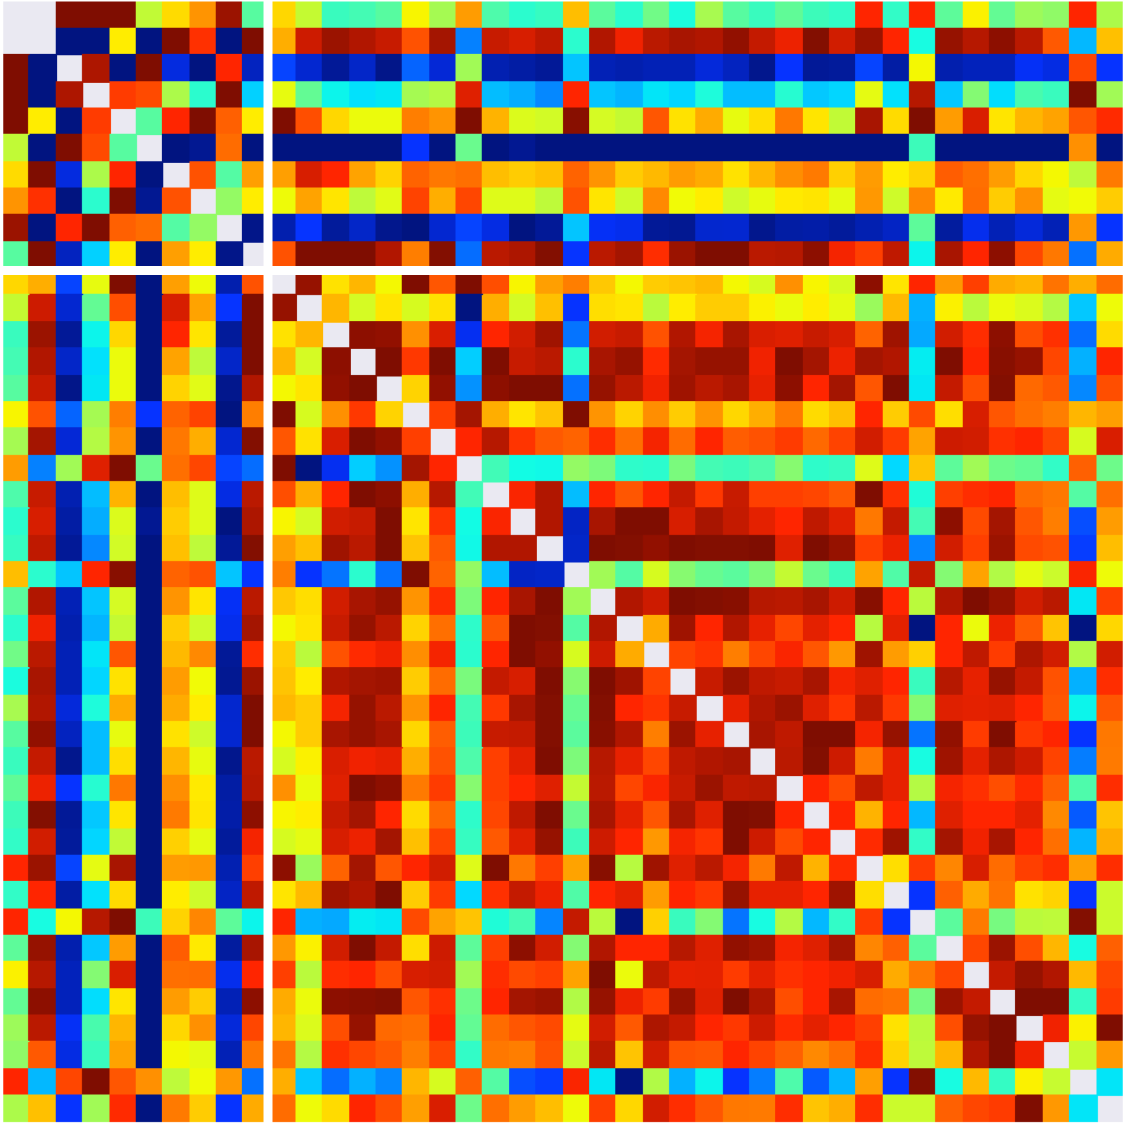
\includegraphics[width=0.45\columnwidth]{Methodology/figures/gt.png}&
  

    
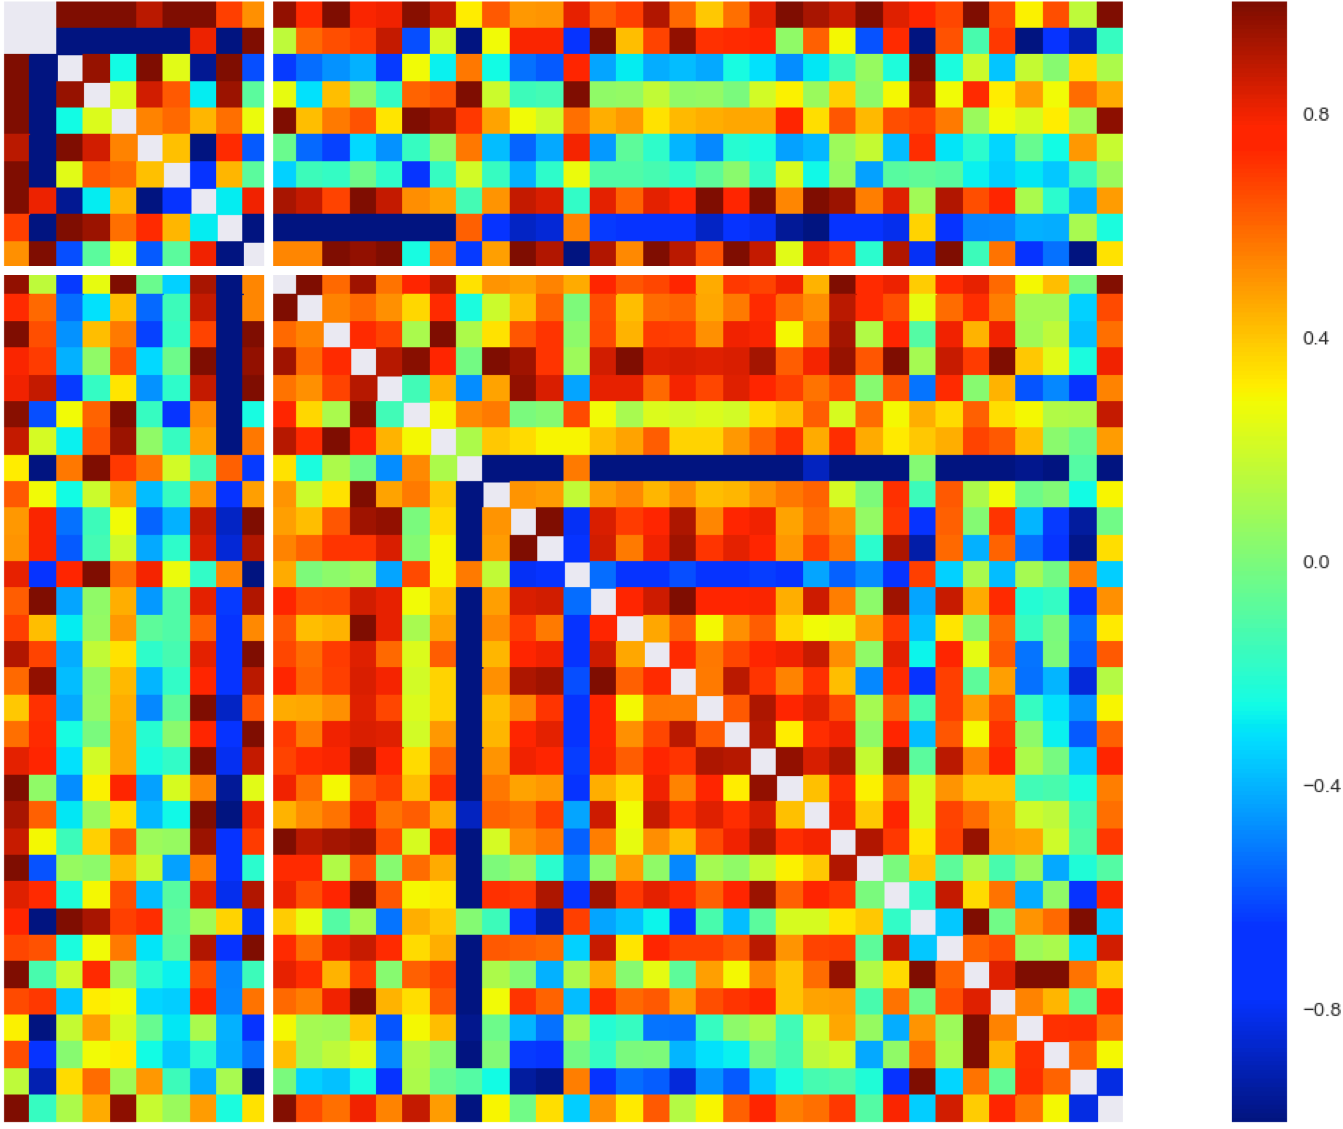
\includegraphics[width=0.54\columnwidth]{Methodology/figures/mmpl.png}&

    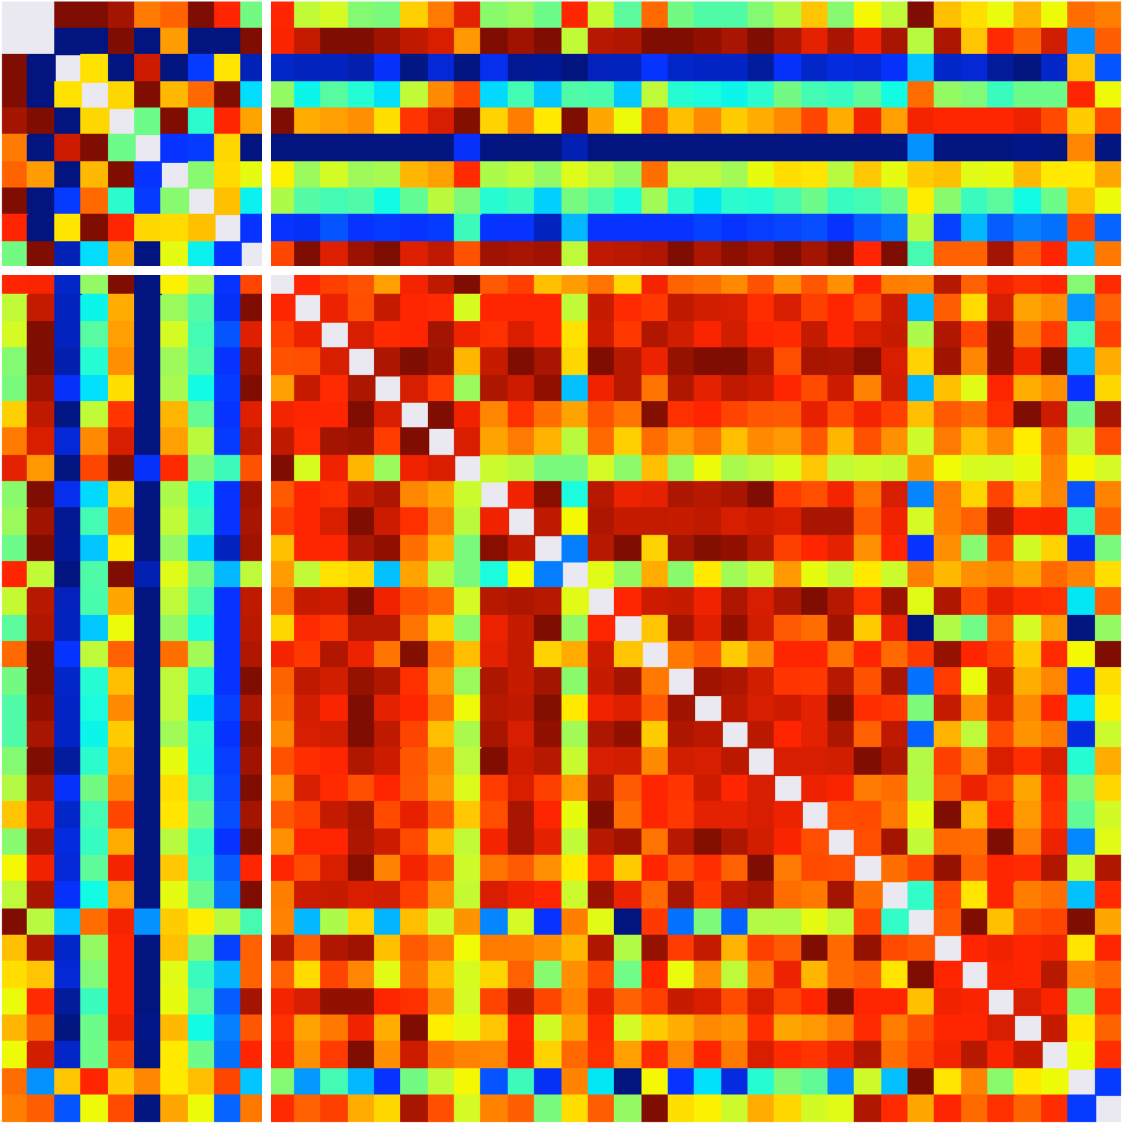
\includegraphics[width=0.45\columnwidth]{Methodology/figures/mrf.png}
\\                                                                        {\small (a) Ground-truth} & {\small (b) MMPL } & {\small (c) MMPL-MRFs} 
  \end{tabular}\vspace{-2mm}
  \caption{\label{fig:consistency} Higher order consistency
    visualization. Figure (a) is calculated
    directly from ground truth labels on test set.
    Figure (b)
    is calculated using predicted labels of MMPL without MRFs on the
    test set.
    In figure (c), we use predicted labels of
    MMPL-MRFs on test set as inputs.}\vspace{0mm}
\end{figure*}

We first select two sectors: nonferrous metal sector, which
contains 10 constituent stocks, and infrastructure sector, which
contains 35 constituent stocks from CSI300 index \footnote{These
  two sectors are selected only because painting many sectors in
  one figure would be too messy to interpret and those two
  sectors have appropriate clique size (number of stocks) for
  visualization. Conclusions from these two sectors also apply to
  other sectors}. We then measure consistency level between each
two of these constituent stocks. In order to capture their
temporal relationship, we propose a novel consistency measure
which is calculated on temporal intervals.
% Let $\C\in\{\text{Nonferrous Metal},\text{Infrastructure}\}$
% denotes one clique. $\by_c=\{\by_i \in \C\}$ denotes a set of
% time-series $\by_i^T=\{y_i^1,y_i^2,...,y_i^T\}$ for all stocks

Let $\by_i^T=\{y_i^1,y_i^2,...,y_i^T\}$ denotes time-series for
stock $i$. $y_i^t\in \{0,1\}$ is the binary price movement label
at time $t$. We segment time-series $\by_i^T$ into
$N=\lceil\frac{T}{P}\rceil$ non-overlapping intervals
$\{y_i^n,y_i^{n+1},...,y_i^{n+P}\}$ with fixed length $P$. For
any two stocks $i$ and $j$, we calculate the difference
$d_{ij}^n=\sum_n^{n+P}{y_i^n}-\sum_n^{n+P}{y_j^n}$ of how many
times positive price movement happen in the $n$th time interval
in each stock. Then the consistency level $c_{ij}$ between stocks
$i$ and $j$ can be calculated as a $\ell_1\text{norm}$:
$$c_{ij}=-\|\mathbf{d}_{ij}\|_1$$
\noindent where
$\mathbf{d}_{ij}=\{d_{ij}^1,d_{ij}^2,...,d_{ij}^N\}$. We
normalize $c_{ij}$ into interval $[-1,1]$. Each entry in
figure~\ref{fig:consistency} denotes a consistency level measure
$c_{ij}$. The larger the $c_{ij}$ is, the higher of consistency
level between stock $i$ and stock $j$, the color of corresponding
entry is closer to red, and vice versa. As we mentioned, the average duration of information
arrival-conduction-integration-release process is 4.04 minutes~\cite{fangyan2012}.
Since which stock is leading at each time interval is elusive, we
set $P=9$ when calculating consistency measures.

As we can see in figure (a), there is a significant red square
area, which means ground-truth heat-map shows strong intra-clique
consistency. This is an evidence that higher-order relationships
do exist within clique of stocks. However, in figure (b), the red
square area is fragmented into many little pieces. The whole
area's color is closer to blue when compared to ground-truth
heat-map, which means that MMPL captures little higher-order consistency.
The reason we still can observe a shape of red square
is that the accuracy of MMPL model on CSI300 is $66.6\%$.
However, we can still conclude that the accuracy of single MMPL
model mainly comes from unary features and it fails to capture
higher order consistency relationships lies in clique of stocks.
On the contrary, even though MMPL-MRFs model's accuracy on CSI300
index is only $2.35\%$ better than MMPL model, we can observe
that heat-map (c) is more close to ground-truth heat-map than
heat-map (b). There is a much clear red square and the number of
small fragments in red area is also less than figure (b). We can
conclude that MMPL-MRFs models learn to utilize both unary
features from MMPL as well as higher-order relationships encoded
in MRFs.

\section{Conclusions}
\label{sec:conc}

Here we show how to model individual stock price predictions without hand-crafted features and encode lead-lag relationships between stocks using weighted higher-order MRFs. A multi-task neural network framework - Multi-task Market Price Learner (MMPL) - is proposed to automatically extract diversified and complementary features from individual stock price sequences. Features learned by MMPL are passed to a binary MRF with a weighted lower linear envelope energy function to utilize intra-clique higher-order consistency between stocks. An efficient latent structural SVM algorithm is designed to learn MRFs in polynomial time. Finally, the MRFs and MMPL are trained end-to-end using the sub-gradient algorithm. Extensive experiments are conducted on three major Chinese stock market indexes, and the proposed MMPL-MRFs achieve the best accuracy on all three indexes.

Our work provides a number of directions for future research. In this work we proposed a multi-task neural network for stock price prediction. While we directly use DARNN as a proof of concept, other, more dedicated architectures are worthy of exploration. Another obvious extension is to apply our method to multi-label MRFs to help with three-class price movement prediction. As well as time series tasks, we can also investigate how the latent SSVM framework performs on computer vision tasks. Another interesting direction is to investigate the implicit relationship between the expert-defined index list and graph RNN~\cite{you2018graphrnn}, which could further help to reduce the domain knowledge required by our framework.

%%
%% The acknowledgments section is defined using the "acks" environment
%% (and NOT an unnumbered section). This ensures the proper
%% identification of the section in the article metadata, and the
%% consistent spelling of the heading.
\begin{acks}
  We would like to thank Stephen Gould very much for explaining
  higer-order MRFs. We would also like to thank Peerajak
  Witoonchart for his explanation of sub-gradient SSVMs
  algorithm.

  We acknowledge data provision and MQD research infrastructure
  support from CMCRC. Li is grateful for funding from the CMCRC.
  This work is also funded by China Hebei Provincial Department
  of Human Resources. Project ID: CL201723.
\end{acks}

%%
%% The next two lines define the bibliography style to be used, and
%% the bibliography file.
\bibliographystyle{ACM-Reference-Format}
\bibliography{Bibs/thesis,Bibs/long,Bibs/scene,Bibs/proposal,Bibs/fin}

%%
%% If your work has an appendix, this is the place to put it.
\appendix

\section{Training Details}
\label{sec:train_detail}

\subsection{Initialization of lower linear envelope}
\label{sec:sup_init}

We assume that the more evenly distributed of $W_c(Y_c)$ where
$c\in\cal C$ on $x$ axis, the more rich representation (number of
linear functions) the energy function should have. In order to
initialize $\btheta$, we first determine the x-coordinate of
sampled points $sp$. Then we sample its y-coordinate from a
uniform distribution ${\cal U}(\text{upbound},\text{upbound}-0.5)$ to add some
randomness in our initialization as well as maintain concavity.
Linear parameters $a_k$ and $b_k$ are later calculated using
those sampled points $sp_k$ and $sp_{k-1}$. At last we encode
$\{a_k,b_k\}_{k=1}^K$ into $\btheta$ using
equation~\eqref{eq:llsvm_param}. This algorithm is summarized in
\algref{alg:init_theta}.

\begin{algorithm}[h]
  \begin{algorithmic}[1]
    \STATE{$gap=\frac{1}{K}$, $a_1={\cal U}(0,1e6)$, $b_1=0$,
      $sp_1=(0,0)$, $w_0=0$, $counter=2$} \FOR{each
      clique $c\in \cal C$} \STATE{Compute weighted clique value
      $w_c=W_c(y_C)$} \IF{$w_c-w_{c-1}>gap$}
    \STATE{$upbound = a_{counter}w_c+b_{counter}$\\
      $sp_{counter}=(w_c,{\cal U}(upbound-0.5,upbound))$\\
      Calculate $a_{counter}$ and $b_{counter}$ using
      $sp_{counter-1}$ and $sp_{counter}$\\
      $counter=counter+1$}
    \ENDIF
    \ENDFOR
    \STATE{If $counter<K$, remaining $a$s and $b$s are all set to
      be $a_{counter}$ and $b_{counter}$} \STATE{Calculate
      $\btheta$ using $\{a_k,b_k\}_{k=1}^K$}
  \end{algorithmic}
  \caption{\label{alg:init_theta} Empirical initialization
    algorithm for $\btheta$}
\end{algorithm}

\subsection{Multi-task training}
\label{sec:multi_train}

To improve accuracy and reduce over-fitting, we add a drop out
layer between input layer and LSTM layer with a ratio of $0.2$.
We also clip and normalize gradients during back-propagation
stage with a maximum norm of $5.0$ to prevent gradient exploding
issue. As pointed out by \citename{lample2016neural}, the
question of ``when should the training schedule switch from one
task to another task?'' or ``should each task be weighted
equally?'' remains open. In our implementation, we follow the
proportional sampling approach described by
\citename{sogaard2016deep}. After a backward pass completed, we
randomly sample a new task as well as its batch data as the next
task to be trained. In practice, we use a proportion of
$[0.25,0.25,0.5]$ for three tasks respectively. This mechanism
helps multi-task model to avoid \emph{Catastrophic Forgetting}
phenomenon which means lower level model forgets learned
knowledge during higher level model back-propagation pass.

Even though we propose an end-to-end training algorithm for MMPL
and MRFs in section~\ref{sec:mmpl}, MRFs inference stage is still
too slow to be trained jointly with MMPL. To overcome this
difficulty, we implement a two stages training procedure. We
first add a \emph{softmax} layer on top of
$\text{DARNN}_{\text{class}}$ and train MMPL separately from
MRFs. We use \emph{Negative Log-likelihood} as the loss function.
At the second stage, after MMPL converge, we remove the
\emph{softmax} layer and re-train it together with MRFs. One
issue we must mention is that, even though we use binary MRFs
which can only predict positive / negative price movement, we
find there is a significant amount of time when stock price
remains no change. We find it benefits the performance a lot if
we treat the classification as a three classes problem rather
than a binary classification problem during the first stage.
Therefore, at the first stage, the \emph{softmax} layer will
output probability for three labels: \emph{negative movement},
\emph{no changes} and \emph{positive movement}. Since binary MRFs
still needs a two dimension input as part of unary energy
function, after the \emph{softmax} layer is removed, we add an
additional linear mapping layer between logits of MMPL and MRFs
at the second stage.

\subsection{End-to-end multi-task RNN-MRFs training}
\label{sec:mrf_train}

\begin{algorithm}[h]
  \begin{algorithmic}[1]
    \STATE{Set $MaxIter = 100$}
    \STATE{ {\bf input} training set $\{\by_i\}_{i=1}^{n}$, regularization constant $C > 0$,
      and tolerance $\epsilon \geq 0$}
    \STATE{Initialize $\btheta$ using \algref{alg:init_theta}}
    \REPEAT \STATE{CCCP Outer Loop}
    \STATE{Set $iter = 0$}
    \FOR{each training example, $i = 1, \ldots, n$}
    \STATE{compute $ \bz_i^*=\argmax_{\mathbf{z} \in \mathcal{Z}}
      \theta \cdot \psi(\mathbf{y}_i,\mathbf{z}) $}
    \ENDFOR

    \STATE{ {\bf initialize} active constraints set ${\cal C}_i = \{ \}$ for all $i$}
    \REPEAT \STATE{CCCP Inner Loop}

    \STATE{solve the quadratic programming problem in
      equation~\ref{eq:mrflssvm_object} with respect to active
      constraints set ${\cal C}_i$ for all $i$ and concavity constraints
      $A\btheta\geq \epsilon$ to get
      $\hat{\btheta}$ and $\hat{\bxi}$}

    \FOR{each training example, $i = 1, \ldots, n$}
    \STATE{compute $\hat{\by_i},\hat{\bz_i} = \argmin_{\by}
      E(\by,\bz; \hat{\btheta}) - \Delta(\by, \bz, \by_i)$}
    \IF{$\hat{\xi}_i + \epsilon \!<\! \Delta(\hat{\by_i},
      \hat{\bz_i}, \by_i) -
      E(\hat{\by_i},\hat{\bz_i}; \hat{\btheta}) + E(\by_i, \bz_i^*; \hat{\btheta})$}
    \STATE{${\cal C}_i \leftarrow {\cal C}_i \cup \{{\by}_i^\star\}$}
    \ENDIF
    \ENDFOR
    \UNTIL{no more violated constraints}
    \STATE{ {\bf return} parameters $\hat{\btheta}$}
    \STATE{Set $iter = iter+1$}

    \UNTIL{$iter\geq MaxIter$}
    \STATE{ {\bf return} parameters $\hat{\btheta}$}
  \end{algorithmic}
  \caption{\label{alg:learning} Learning lower linear envelope
    MRFs with latent variables.}
\end{algorithm}

With converged MMPL and MRFs at hand, now we can go forward to
train them in an end-to-end manner. We only include pairwise
energy function through section~\ref{sec:srp} and
section~\ref{sec:opt} to show a general application of our
proposed algorithm. In the case of Chinese stock market, to our
best knowledge there is no public available definition of
pairwise relationship between stocks. Therefore, in our
implementation we only use unary and higher order energy
function. Each stock is then treated as a node in MRFs and each
stocks group which has lead-lag relationships is treated as a
maximum clique in MRFs. One benefit of MRFs clique is that we can
embed domain expert knowledge about industry classification as
maximum cliques into our model. We choose to use Tonghuashun
industry classification \cite{ths} in our model. One subtle but
crucial detail about modeling lead-lag effect lies in
equation~(\ref{eqn:potential2}). Recall that $W_{\!c}(\by_c) =
\sum_{i \in c} w_i y_i$ with $w^c_i \geq 0$ and $\sum_{i \in c}
w^c_i = 1$ which are weights for stocks in each clique.
Therefore, leading stocks should have a higher weights while
lagging stocks should have lower weights. In our implementation,
we use constituents' weight defined in CSI200, CSI500 and CSI300
as their weights in equation~(\ref{eqn:potential2}) and normalize
them to ensure the summation equals $1$.

\end{document}
\endinput
%%
%% End of file `sample-sigconf.tex'.
